% Tamaño de letra.
\documentclass[12pt,titlepage]{report}

%------------------------------ Paquetes ----------------------------------

% Paquetes:

%Para comentarios multilínea.
\usepackage{verbatim}

% Para tener cabecera y pie de página con un estilo personalizado.
\usepackage{fancyhdr}

% Codificación UTF-8
\usepackage[utf8]{inputenc}

% Castellano.
\usepackage[spanish]{babel}

% Tamaño de página y márgenes.
\usepackage[a4paper,headheight=16pt,scale={0.75,0.8},hoffset=0.5cm]{geometry}

% Para poder agregar notas al pie en tablas:
%\usepackage{threeparttable}

% Tipo de letra Helvetica (Arial).
%\usepackage{helvet}
%\renewcommand\familydefault{\sfdefault}

% Gráficos:

% Para incluir imágenes, el siguiente código carga el paquete graphicx
% según se esté generando un archivo dvi o un pdf (con pdflatex).

% Para generar dv.
%\usepackage[dvips]{graphicx}

% Para generar pdf.
\usepackage[pdftex]{graphicx}
\pdfcompresslevel=9

\usepackage{pdfpages}

%
% Directorio donde están las imagenes.
%
%\newcommand{\imgdir}{includes}
%\graphicspath{{\imgdir/}}

%------------------------------ ~paquetes ---------------------------------

%------------------------- Inicio del documento ---------------------------

\begin{document}

% ---------------------- Encabezado y pie de página -----------------------

% Encabezado: sección a la derecha.
% Pie de página: número de página a la derecha.

\pagestyle{fancy}
\renewcommand{\sectionmark}[1]{\markboth{}{\thesection\ \ #1}}
\lhead{}
\chead{}
\rhead{\rightmark}
\lfoot{}
\cfoot{}
\rfoot{\thepage}

% ---------------------- ~Encabezado y pie de página ----------------------

% -------------------------- Título y autor(es) ---------------------------

\title{Información en las organizaciones}
\author{}

% -------------------------- ~Título y autor(es) --------------------------

% ------------------------------- Carátula --------------------------------

\begin{titlepage}

\thispagestyle{empty}

% Logo facultad más pie de la figura.
\begin{center}

\includegraphics[scale=0.55]{./Images/fiuba}\\
\large{\textsc{Universidad de Buenos Aires}}\\
\large{\textsc{Facultad De Ingeniería}}\\
\small{Año 2012 - 1\textsuperscript{er} Cuatrimestre}
\end{center}

\vfill

% Título central.
\begin{center}

\Large{\underline{\textsc{Información en las organizaciones (71.13)}}}

\vfill

% Tabla de integrantes.

\Large{\underline{\textsc{Trabajo Práctico}}}
\vfill

\Large\underline{Ayudante: Licenciada Paez} \linebreak\linebreak
\Large\underline{Integrantes Grupo 2} \linebreak\linebreak

% Separación entre columnas.
\large\addtolength{\tabcolsep}{-3pt}
% Tres columnas con alineación centrada.
\begin{tabular}{|| c | c | c ||}
\hline
\textbf{Apellido, Nombre} & \textbf{Nro. Padrón} & \textbf{E-mail} \\
\hline
Berrilio, Pablo & 88812 & pabloberrilio@gmail.com \\
\hline
Bukaczewski, Verónica & 86954 & vero13@gmail.com \\
\hline
De Antoni, Matías & 88506 & mdeantoni87@gmail.com \\
\hline
Garbarini, Lucía & 88300 & lu.teddy@gmail.com\\
\hline
Invernizzi, Esteban Ignacio & 88817 & invernizzie@gmail.com\\
\hline
Mouso, Nicolás Gastón & 88528 & nicolasgnr@gmail.com \\
\hline
Ygounet, Guido N. & 88246 & gygounet@gmail.com \\
\hline
Zelechowski, Sergio & 86651 & sergiozz123@gmail.com \\
\hline
Moreno Salas, Josué Fabio & Intercambio & josue.nalgarito@gmail.com \\
\hline
\end{tabular}
\end{center}

\vfill

\hrule
\vspace{0.2cm}

% Pie de página de la carátula.
\noindent\small{71.13 - Información en las organizaciones \hfill Grupo 2}

\end{titlepage}

% ------------------------------- ~Carátula -------------------------------

% -------------------------------- Índice ---------------------------------

% Hago que las páginas se comiencen a contar a partir de aquí.
\setcounter{page}{1}

% Índice.
\tableofcontents
\newpage

% -------------------------------- ~Índice --------------------------------

% ----------------------------- Inicio del tp -----------------------------

\chapter*{Enunciado}
\begin{center}
 
\includegraphics[keepaspectratio=true]{./Images/pagina1-guia.png}
 % pagina1-guia.png: 632x889 pixel, 96dpi, 16.72x23.52 cm, bb=0 0 474 667
\end{center}
\includepdf[pages=2-11, scale=0.9, pagecommand={\thispagestyle{empty}}]{./2012_GuiaTPCampo.pdf}

\part{Memoria Descriptiva de la Empresa. Historial de la misma. Resumen de los Sistemas de
información de la Empresa.}

\chapter{Elección de la empresa}
% TABLA COMPARATIVA
\section{Tabla comparativa de empresas}
\begin{center}
\small\addtolength{\tabcolsep}{-5pt}
\begin{tabular}{|| c || c || c | c | c | c | c ||}
\hline
\hline
T\'{e}rminos & Peso & Empresa 1 & Empresa 2 & Empresa 3 & Empresa 4 & Empresa 5\\
\hline
Contacto   & 10 & 9 & 8 & 10 & 10 & 8 \\
\hline
Ubicaci\'{o}n & 7 & 6 & 10 & 5 & 6 & 7 \\
\hline
Tama\~{n}o & 8 & 9 & 8 & 8 & 3 & 8 \\
\hline
Disp. de info. & 10 & 9 & 6 & 10 & 8 & 8 \\
\hline
Centralizaci\'{o}n & 4 & 8 & 8 & 7 & 6 & 8 \\
\hline
\hline
Totales & - & 326 & 306 & 327 & 270 & 305 \\
\hline
\end{tabular}
\end{center}

%\pagebreak

% ELECCIÓN FINAL.

\section{Elección de la empresa}
Se eligió la empresa \textbf{Empresa X}, principalmente por haber obtenido el mejor puntaje según el criterio de comparación elegido. La buena calidad del contacto y la exelente disponibilidad de información situa a esta empresa por encima de otras propuestas.

\pagebreak

\chapter{Actividad de la empresa IEP De Iluminación}
\begin{center}
 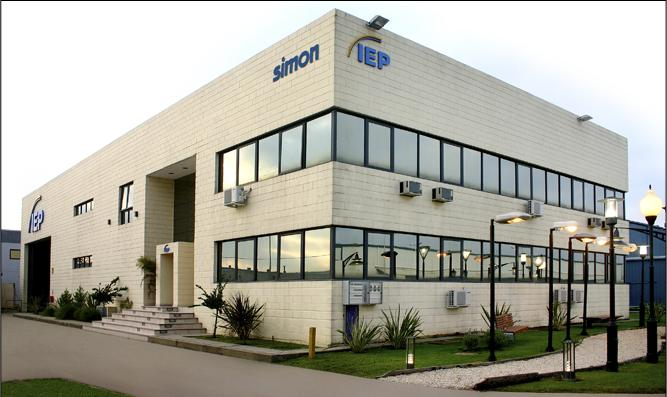
\includegraphics[scale=0.75]{./Images/iep-instalacion.png}
\end{center}
\section{Introducci\'on}
\subsection{Descripción}
Es una empresa multinacional dedicada a la fabricación y comercialización de luminarias, farolas, columnas y soportes, que ofrece soluciones de excelente calidad luminotécnica en Alumbrado Público, Áreas Verdes, Alumbrado Industrial, Alumbrado Interior, Alumbrado de Jardín, Iluminación con Sumergibles y Leds.

\subsection{Ubicación}
La empresa se encuentra ubicada en las afueras de la Ciudad de Buenos Aires, m\'as precisamente en el conurbano bonaerense en el kil\'ometro 37.5 del ramal Escobar de la Ruta Panamericana. A pesar de encontrarse a aproximadamente 
40 kil\'ometros de la Capital Federal, es relativamente f\'acil y r\'apido llegar hasta la f\'abrica.

\subsection{Historia}
En el año 1922 Industrias Electrotécnicas Puig (IEP) se especializaba en la fabricación de aparatos reflectores para alumbrado en la española ciudad de Barcelona.
En el año 1966 pasa a formar parte del Grupo Simon, un holding de empresas del mercado eléctrico español con visionaria expansión hacia a los cinco continentes.
A principios de la década del 90 adapta nuevamente su estructura y su imagen, empezando a conocérsela como IEP DE ILUMINACIÓN.
Es en el año 1998 que IEP DE ILUMINACIÓN llega a la Argentina, convirtiéndose en el lapso de 12 años en la principal responsable de la comercialización de luminarias para toda América del Sur. 
Como en todo proceso de expansión y desarrollo, el Grupo Simon fue incorporando nuevos centros de producción y filiales en Latinoamérica (Argentina, Brasil y México), en Europa (Francia, Reino Unido, Irlanda, Bélgica, Holanda, Noruega, Suiza, Polonia), en África (Marruecos y Egipto) y en Asia (China, India, Rusia, Turquía) para poder llegar con mayor rapidez y eficiencia operativa a todos sus mercados.
En la actualidad cuenta con 24 empresas coordinadas desde su sede central en Barcelona (España) y su presencia mundial alcanza a más de 50 países. Centra sus actividades en el ámbito de la instalación eléctrica con diversas líneas de productos: material eléctrico y protección de circuitos, iluminación, domótica, conexiones para voz y datos, canalizaciones y electrónica. Las más recientes incorporaciones en su línea de negocios comprenden el mobiliario urbano y la seguridad. El primero por su relación con los espacios de iluminación urbana y el segundo porque las innovaciones aplicadas en este campo también incluyen material eléctrico.

\subsubsection{En Argentina}
Durante sus primeros años de actividad en el país, la empresa contó con planta de producción en la localidad de Munro (Buenos Aires) y oficinas comerciales en San Isidro (Buenos Aires), pero el creciente aumento de los volúmenes de venta fundados en la producción de luminarias de avanzada tecnología y diseños de vanguardia, demandó la instalación de una planta fabril de mayor tamaño y capacidad productiva.
Así, posicionada en el ámbito local como la empresa “Líder en Innovación Tecnológica”, IEP DE ILUMINACIÓN cuenta desde el año 2005 con instalaciones propias dentro del Centro Industrial Garín (Buenos Aires), garantizando rapidez operativa y de organización al reunir en un mismo lugar tanto sus áreas Comerciales como las de Producción y Almacenamiento.

\section{Filosof\'ia de la empresa}

\subsection{Misi\'on}

La misi\'on de la empresa consiste en operar un sistema rentable que les permita satisfacer las necesidades actuales y potenciales del mercado luminot\'ecnico, 
ofreciendo productos y servicios con verdadero valor agregado, a fin de construir relaciones fuertes y a largo plazo.

\subsection{Visi\'on}

La empresa define su visi\'on de la siguiente forma:\\
Ser considerada la empresa de iluminaci\'on m\'as pujante convirtiendonos en el proveedor preferido por el mercado luminot\'ecnico al ofrecer los mejores 
productos y servicios del rubro.
 
\section{Estructura de la empresa}

\subsection{Organigrama}
A continuación se presenta el organigrama completo de la empresa. Ver imagen \ref{organigramaIEP}

\begin{figure}[h!]
  \centering
  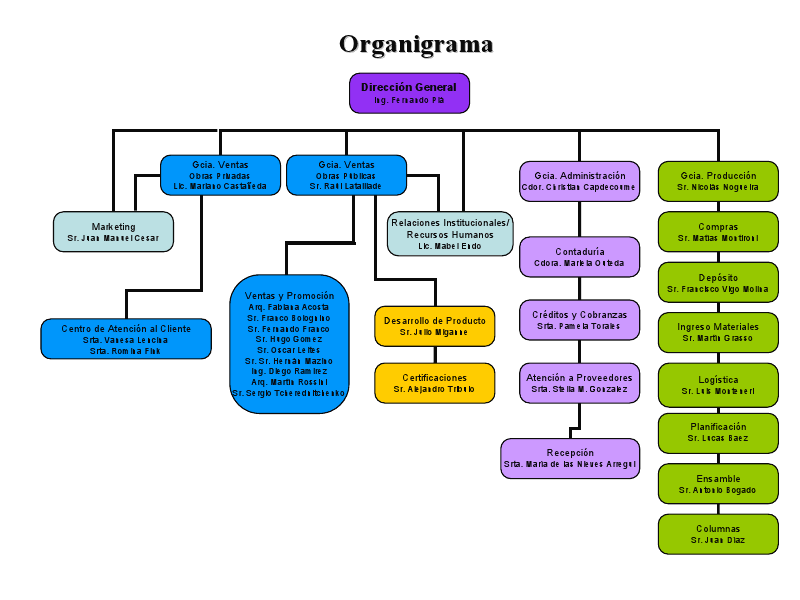
\includegraphics[scale=0.55]{./Images/organigrama.png}
  \caption{Organigrama IEP}\label{organigramaIEP}
\end{figure}

\part{Sistemas de Información teóricos dados en las Clases Prácticas. Cursogramas teóricos.
Formularios teóricos de los sistemas de información estudiados. Normas de control interno
generales y particulares.}

\chapter{Circuito Pago a Proveedores}
\section{Cursograma Pagos a Proveedores}
\begin{center}
 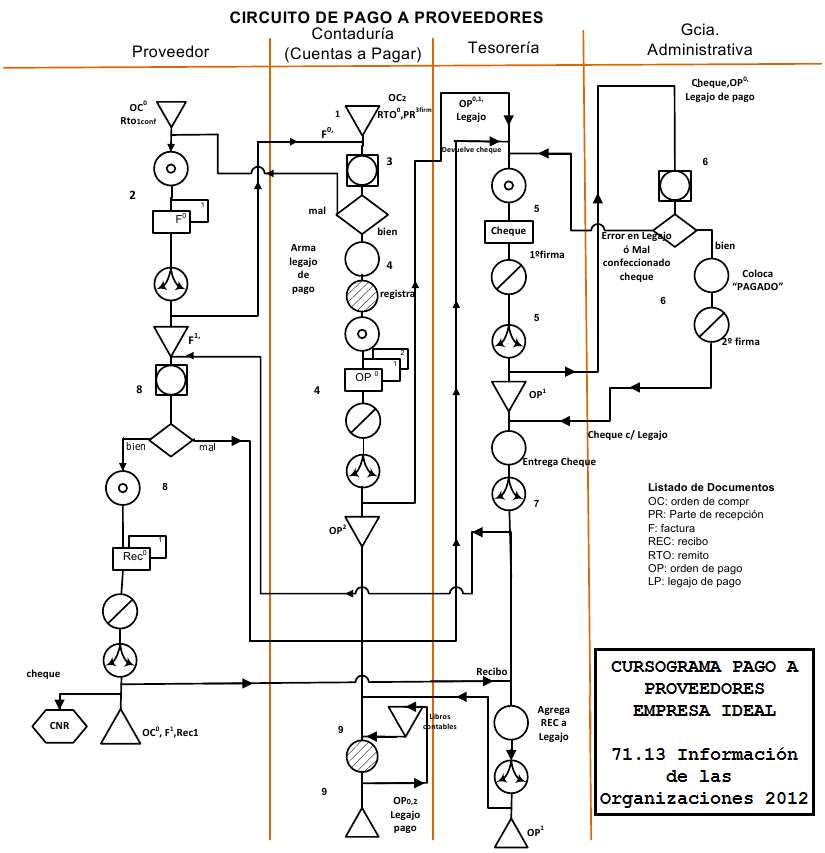
\includegraphics[scale=0.7,keepaspectratio=true]{./Circuitos-Teoricos/Pago-a-Proveedores/Images/cursograma-pago-a-proveedores.png}
 % cursograma-pago-a-proveedores.png: 587x630 pixel, 96dpi, 15.53x16.67 cm, bb=0 0 440 472
\end{center}

\section{Procedimiento de Pagos a Proveedores}
\begin{center}
 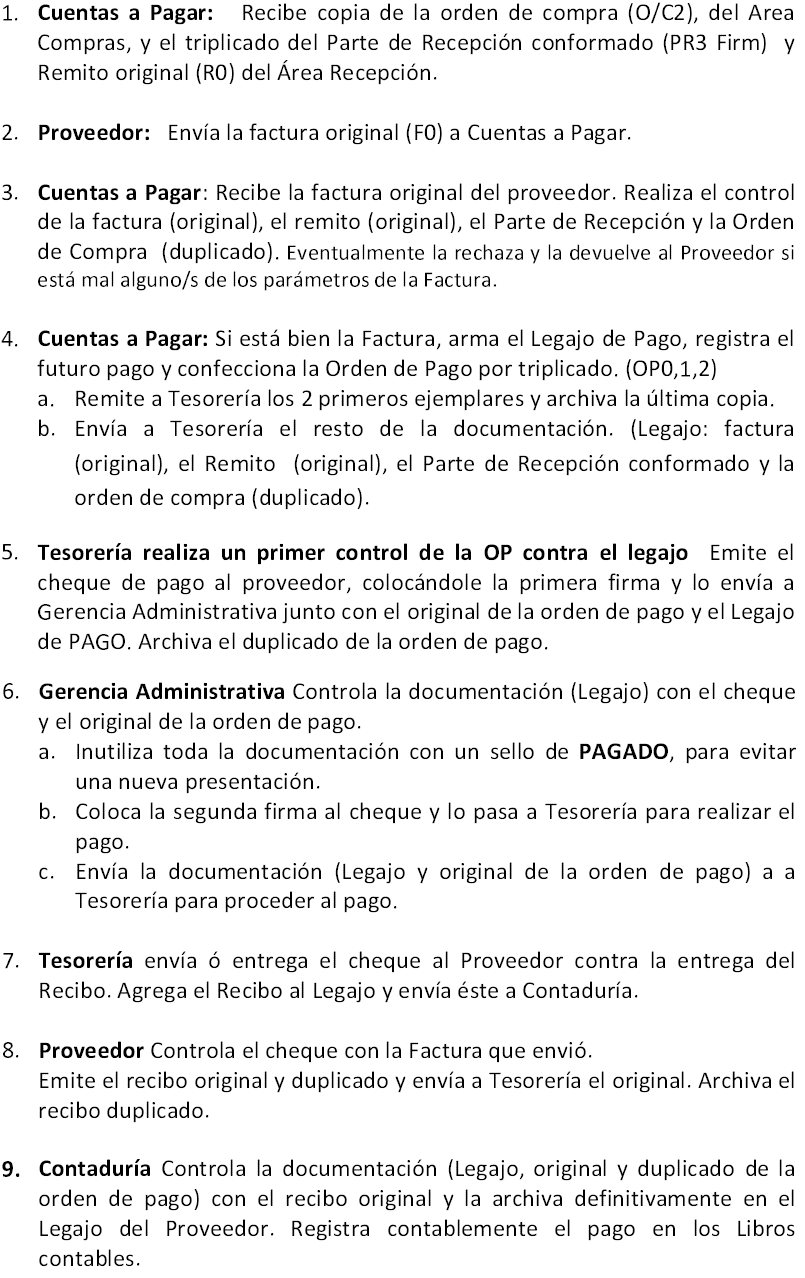
\includegraphics[scale=0.7,keepaspectratio=true]{./Circuitos-Teoricos/Pago-a-Proveedores/Images/procedimiento-pago-a-proveedores.png}
 % procedimiento-pago-a-proveedores-1.png: 805x927 pixel, 96dpi, 21.30x24.52 cm, bb=0 0 604 695
\end{center}

\section{Cursograma de Pagos (con numeración para el manual)}
\subsection{Manual del Cursograma de Pagos}

\begin{center}\textbf{Sectores intervinientes}\end{center}
\begin{itemize}
  \item Proveedor
  \item Contaduría (Cuentas a pagar)
  \item Tesorería
  \item Gcia. Administrativa
\end{itemize}

\begin{center}
  \textbf{Emisión de Documentos}
  
\includegraphics{./Images/Simbolos/simbolo-Emision-de-Documentos.png}
\end{center}
\begin{enumerate}
  \item Proveedor emite factura, original y copia
  \item Proveedor emite recibo del pago, en original y duplicado.
  \item Cuentas a pagar, de acuerdo a la factura recibida, confecciona la Orden de Pago por triplicado.
  \item Tesorería emite cheque de pago a proveedor.
\end{enumerate}

\begin{center}
  \textbf{Documentos}
  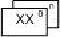
\includegraphics{./Images/Simbolos/simbolo-Documentos.png}
\end{center}
\begin{enumerate}
  \item Factura (F).
  \item Recibo (REC)
  \item Orden de pago (OP).
  \item Cheque
\end{enumerate}

\begin{center}
  \textbf{Distribución}
  
\includegraphics{./Images/Simbolos/simbolo-Distribucion.png}
\end{center}
\begin{enumerate}
  \item Proveedor distribuye factura original a cuentas a pagar, y conserva el duplicado.
  \item Proveedor distribuye recibo original a Tesorería, conserva el duplicado.
  \item Cuentas a Pagar distribuye las órdenes de pago. Original y duplicado a Tesorería, conserva el triplicado.
  \item Tesorería distribuye cheque, orden de pago original y legajo de pago a Gcia. Administrativa.
  \item Tesorería distribuye cheque a proveedor.
  \item Tesorería distribuye  Recibo y Legajo a Contaduría.
\end{enumerate}

\begin{center}
  \textbf{Firma}
  
\includegraphics{./Images/Simbolos/simbolo-Firma.png}
\end{center}
\begin{enumerate}
  \item Proveedor firma recibo.
  \item Cuentas a Pagar firma las órdenes de pago.
  \item Tesorería pone la primera firma en el cheque.
  \item Gcia. administrativa pone la segunda firma en el cheque.
\end{enumerate}

\begin{center}
  \textbf{Almacenamiento Transitorio}
  
\includegraphics{./Images/Simbolos/simbolo-Almacenamiento-Transitorio.png}
\end{center}
\begin{enumerate}
  \item Cuentas a Pagar almacena OC2, RTO0 y PR3firm .
  \item Cuentas a Pagar almacena OP2.
  \item Cuentas a Pagar almacena libros contables.
  \item Tesorería almacena OP1.
\end{enumerate}

\begin{center}
  \textbf{Control y verificación}
  
\includegraphics{./Images/Simbolos/simbolo-Control-y-Verificacion.png}
\end{center}
\begin{enumerate}
  \item Proveedor controla el cheque con la factura que envió, para verificar el cumplimiento del pago de la misma, verificando el monto y el plazo de pago.
  \item Cuentas a Pagar realiza control de factura, remito, parte de recepción y la orden de compra, verificando que la factura haya sido correctamente confeccionada, y que tanto ésta última como el remito y el parte de recepción referencien a la orden de compra en cuestión. 
  \item Gcia. administrativa controla el legajo con el cheque y el original de la orden de pago, verificando que el cheque haya sido correctamente confeccionado, para el proveedor en cuestión y con el monto correcto.
\end{enumerate}

\begin{center}
  \textbf{Decisión}
  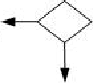
\includegraphics{./Images/Simbolos/simbolo-Decision.png}
\end{center}
\begin{enumerate}
  \item Proveedor controla cheque contra factura, si está bien emite recibo, caso contrario devuelve cheque a Tesorería.
  \item Cuentas a Pagar controla la factura, si está bien confecciona OP, sino la devuelve al proveedor.
  \item Gcia. administrativa controla legajo, OP y cheque, si está bien coloca PAGADO y firma el cheque, caso contrario devuelve la documentación a Tesorería.
\end{enumerate}

\begin{center}
  \textbf{Almacenamiento definitivo}
  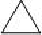
\includegraphics{./Images/Simbolos/simbolo-Almacenamiento-Definitivo.png}
\end{center}
\begin{enumerate}
  \item Proveedor almacena definitivamente OC0, F1 y Rec1
  \item Cuentas a Pagar almacena definitivamente OP0, 2, y Legajo de pago.
  \item Tesorería almacena definitivamente OP1
\end{enumerate}

\begin{center}
  \textbf{Operación}
  
\includegraphics{./Images/Simbolos/simbolo-Operacion.png}
\end{center}
\begin{enumerate}
  \item Cuentas a Pagar arma legajo de pago.
  \item Tesorería entrega cheque.
  \item Tesorería agrega el recibo al legajo de pago.
  \item Gcia. administrativa coloca “Pagado” inutilizando toda la documentación, para evitar nueva presentación.
\end{enumerate}

\begin{center}
  \textbf{Registro}
  
\includegraphics{./Images/Simbolos/simbolo-Registro.png}
\end{center}
\begin{enumerate}
  \item Cuentas a Pagar registra la compra en la cta. cte. proveedores.
  \item Cuentas a Pagar registra contablemente el pago en los libros contables. 
\end{enumerate}

\begin{center}
  \textbf{Circuito no relevado}
  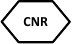
\includegraphics{./Images/Simbolos/simbolo-CNR.png}
  % simbolo-CNR.png: 73x44 pixel, 96dpi, 1.93x1.16 cm, bb=0 0 55 33
\end{center}
\begin{enumerate}
  \item Cobranzas (circuito del proveedor).
\end{enumerate}

\pagebreak
\section{Formularios de Pagos a Proveedores}
\subsection{Orden de Pago} 

\begin{center}
 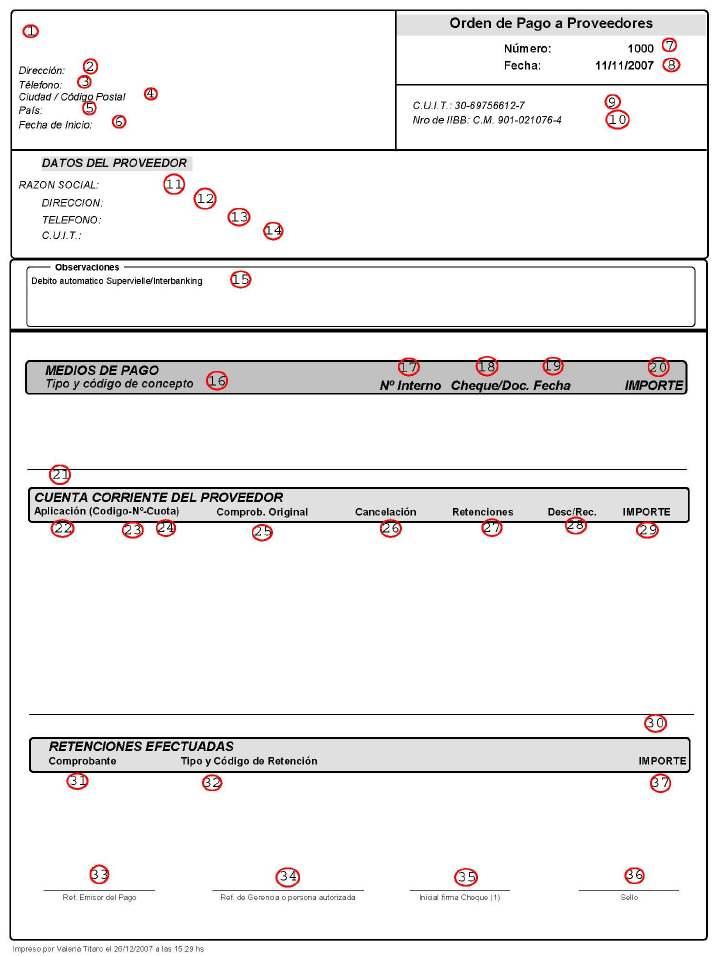
\includegraphics[scale=0.8,keepaspectratio=true]{./Circuitos-Teoricos/Pago-a-Proveedores/Images/orden-de-pago.png}
 % orden-de-pago.png: 721x956 pixel, 96dpi, 19.07x25.29 cm, bb=0 0 541 717
\end{center}

\pagebreak
\begin{itemize}
  \item \textbf{Objetivo:} Con este documento se respalda la emisión del pago que se realizará al proveedor.
Mediante este documento se notifica a los sectores que lo reciben de la existencia y autorización
del pago.
  \item \textbf{Alcance:} Es un documento interno a la empresa.
  \item \textbf{Emisor:} Contaduría.
  \item \textbf{Cantidad de Copias Emitidas:} Original y 2 copias.
  \item \textbf{Sector receptor:} Tesorería.
\end{itemize}

\subsubsection{Descripción}
\begin{center}
 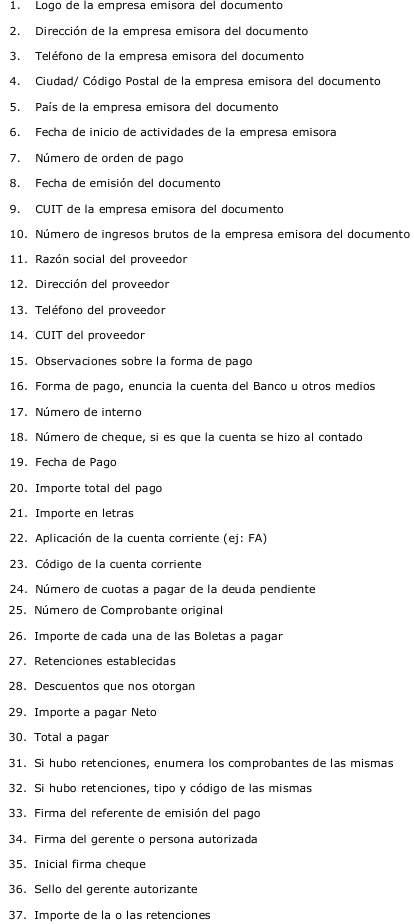
\includegraphics[keepaspectratio=true]{./Circuitos-Teoricos/Pago-a-Proveedores/Images/descripcion-orden-de-pago.png}
 % descripcion-pago-a-proveedores.png: 414x595 pixel, 96dpi, 10.95x15.74 cm, bb=0 0 310 446
\end{center}

\pagebreak
\subsection{Cheque}
\begin{center}
 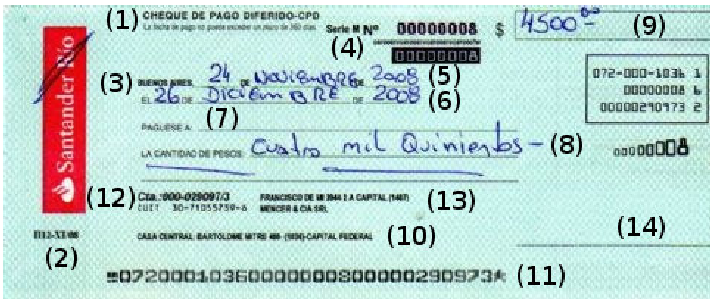
\includegraphics[scale=0.9,keepaspectratio=true]{./Circuitos-Teoricos/Pago-a-Proveedores/Images/cheque.png}
 % cheque.png: 713x304 pixel, 96dpi, 18.86x8.04 cm, bb=0 0 535 228
\end{center}

\begin{itemize}
  \item \textbf{Objetivo:} Con este documento se efectúa el pago. Se entrega al proveedor, y éste por intermedio de un depósito bancario o por ventanilla, obtiene el efectivo que el cheque representa.
  \item \textbf{Alcance:} Es un documento externo a la empresa.
  \item \textbf{Emisor:} Tesorería.
  \item \textbf{Cantidad de Copias Emitidas:} Original.
  \item \textbf{Sector receptor:} Gerencia Administrativa.
\end{itemize}

\subsubsection{Descripción}
\begin{center}
 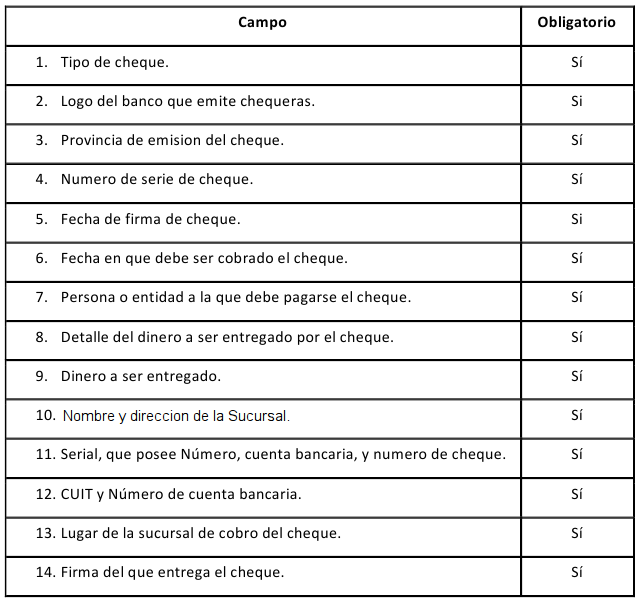
\includegraphics[scale=0.9,keepaspectratio=true]{./Circuitos-Teoricos/Pago-a-Proveedores/Images/descripcion-cheque.png}
 % descripcion-cheque.png: 640x366 pixel, 96dpi, 16.93x9.68 cm, bb=0 0 480 274
\end{center}

\pagebreak
\section{Normas de control interno generales y específicas de Pagos a Proveedores}
\begin{enumerate}
  \item \textbf{Separación de funciones:}
El manejo de los fondos no debe estar a cargo de la misma persona que realiza la registración.  No es conveniente que el cajero realice la registración contable de donde surge el saldo por el cual es responsable, aunque es posible que para su control y para confeccionar las rendiciones que eleva al área contable tenga que efectuar algunas anotaciones.   En el caso particular de los Pagos, la liquidación y autorización debe ser realizada por una persona responsable ajena a Tesorería.
  \item \textbf{Concentración de la responsabilidad:}
Una sola persona será responsable de la custodia y del manejo de fondos, esa persona suele ser el Tesorero.
  \item \textbf{Separación total de los fondos:}
Para un control eficaz de los fondos es recomendable que los provenientes de cobranzas estén separados de los destinados a pagos,  por lo tanto, los valores que tienen origen en las cobranzas se depositaran en su total en la cuenta corriente bancaria y los pagos se efectuaran mediante cheques emitidos contra esa cuenta bancaria.
  \item \textbf{Rotación del personal:}
De manera que se puedan detectar posibles errores en el sistema.  Además, es aconsejable que este personal tome sus vacaciones anuales y que otra persona de la organización esté capacitada para realizar su reemplazo, como así también en casos de enfermedad o egreso del personal.  Los reemplazos se realizaran con personal ajeno al sector y que no tenga amistad o subordinación directa con el reemplazado.
  \item \textbf{Contabilización de las operaciones:}
De manera que permitan el control de las mismas y la consistencia con la información de otros sectores, por ejemplo, total de débitos o créditos en cuentas de terceros.  La registración estará respaldada por la documentación correspondiente.
  \item \textbf{Arqueos sorpresivos:}
Se realizan para verificar si los valores en existencia coinciden con los que surgen de la registración contable.
  \item \textbf{Conciliación bancaria}
\end{enumerate}

\subsection{Normas Específicas}
\begin{itemize}
  \item \textbf{Uso del Cheque:}
  \begin{itemize}
    \item Permite disminuir el riesgo que implica la tenencia de dinero en efectivo.
    \item Ejerce un mejor control sobre los pagos debido a que se podrán conciliar con el resumen bancario.
    \item Deben tomarse en cuenta las distintas modalidades que permite la legislación vigente: Ley 24.452 (Ley de Cheques).
    \item Los cheques deben ser firmados por dos responsables de la organización.
    \item Los cheques que se anulen deben quedar adheridos a la libreta de cheques o destruirse el ángulo inferior derecho donde se firma o en la parte donde figura su numeración.
  \end{itemize}


Con esta forma se persiguen dos finalidades:
  \begin{itemize}
    \item Que exista un control reciproco entre los firmantes y de esta manera detectar errores antes de que el pago se haga efectivo. Esto implica que los dos responsables que firman el cheque efectúen una revisión de la documentación respaldatoria y la inicialicen, puesto que de lo contrario esta norma no tendrá sentido.
    \item Se evita que una sola persona pueda disponer del uso indiscriminado de los fondos, con el consecuente riesgo que ello implica.
  \end{itemize}

  \item \textbf{Pago amparado con la totalidad de los comprobantes y anulación de los mismos:}
En el momento de confeccionar el cheque, la persona responsable tendrá a la vista la
documentación respaldatoria que le da origen y se le colocará el sello de “Pagado” y el
número del cheque con el que se efectúo el pago con el objeto de que no vuelva a ser
presentada para justificar o respaldar otro pago. Quienes firmen el cheque deberán
controlar que se cumpla con estos aspectos.
  \item \textbf{Existencia de fondo fijo o caja chica:}
Tendrá un monto estipulado previamente para realizar los pagos menores en efectivo, estará
a cargo de una persona responsable y su reposición se efectuara periódicamente mediante
la emisión de un cheque previa presentación de los comprobantes que respalden los pagos
efectuados.
  \item \textbf{Pagos de sueldos y jornales:}
Es importante que exista una separación de tareas entre quien controla la asistencia, quien
prepara la liquidación de los haberes y quienes efectúa el pago. En este caso, es de
especial interés la seguridad del movimiento de fondos para el pago (seguros de dinero en
transito, traslado por empresas especializadas, etc.). El pago al empleado se realiza previa
identificación y contra la entrega del recibo firmado.
\end{itemize}

\chapter{Circuito Producci\'on}
\section{Cursograma Producci\'on}
\begin{center}
 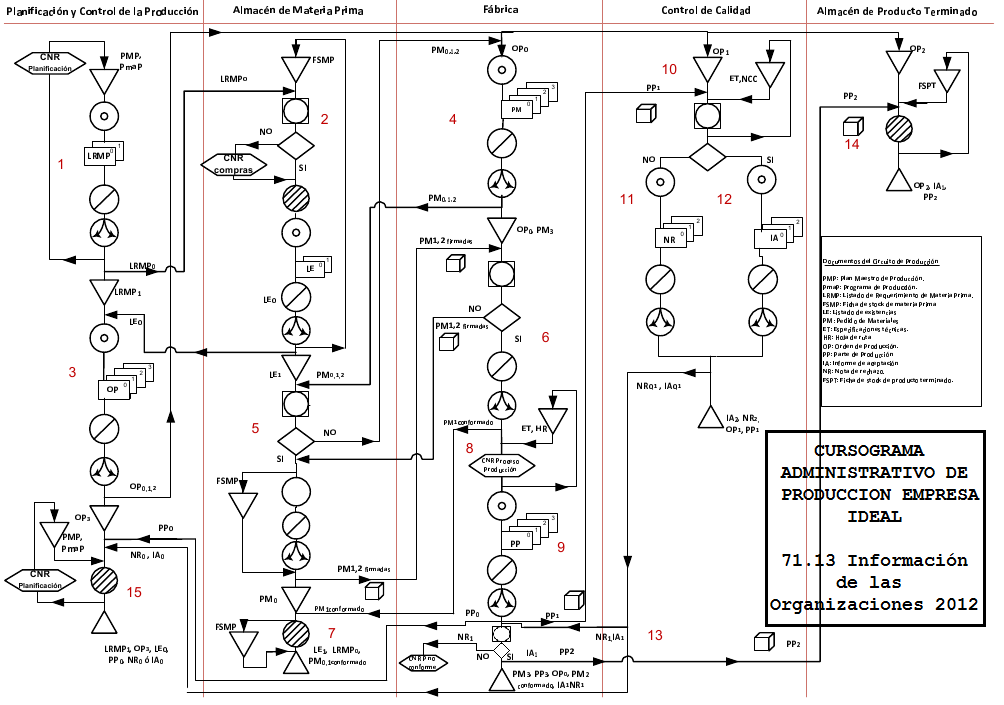
\includegraphics[angle=90,scale=0.95,keepaspectratio=true]{./Circuitos-Teoricos/Produccion/Images/cursograma-produccion.png}
 % cursograma-produccion.png: 1004x705 pixel, 96dpi, 26.56x18.65 cm, bb=0 0 753 529
\end{center}

\section{Procedimiento de Producci\'on}
\begin{center}
 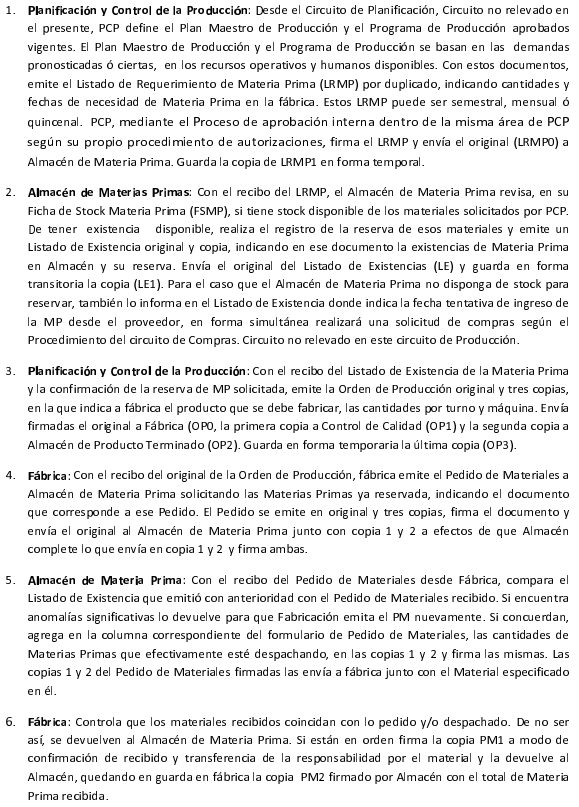
\includegraphics[keepaspectratio=true]{./Circuitos-Teoricos/Produccion/Images/procedimiento-produccion.png}
 % procedimiento-produccion.png: 579x807 pixel, 96dpi, 15.32x21.35 cm, bb=0 0 434 605
\end{center}
\begin{center}
 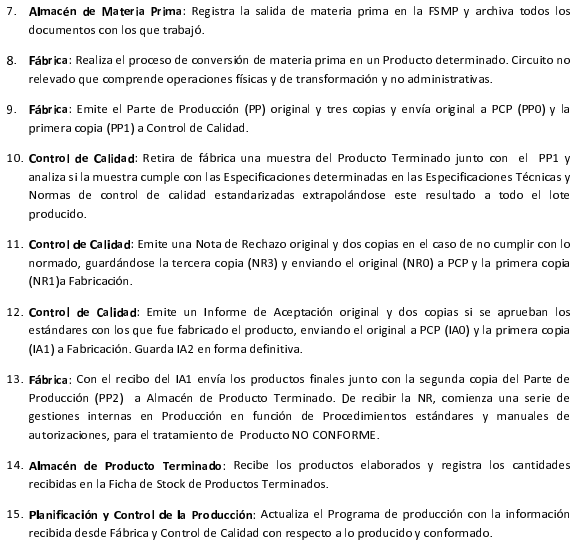
\includegraphics{./Circuitos-Teoricos/Produccion/Images/procedimiento-produccion-2.png}
 % procedimiento-produccion-2.png: 576x545 pixel, 96dpi, 15.24x14.42 cm, bb=0 0 432 409
\end{center}

\pagebreak
\section{Cursograma de Producci\'on (con numeración para el manual)}
\subsection{Manual del Cursograma de Producci\'on}

\begin{center}\textbf{Sectores intervinientes}\end{center}
\begin{itemize}
  \item Planificaci\'on y Control de Producci\'on.
  \item Almac\'en de Materia Prima.
  \item F\'abrica.
  \item Control de Calidad.
  \item Almac\'en de Producto Terminado.
\end{itemize}

\begin{center}
  \textbf{Documentos}
  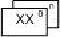
\includegraphics{./Images/Simbolos/simbolo-Documentos.png}
\end{center}
\begin{enumerate}
  \item Listado de Requerimientos de Materia Prima (LRMP).
  \item Orden de Producci\'on (OP).
  \item Listado de Existencia (LE).
  \item Pedido de Materiales (PM).
  \item Parte de Producci\'on (PP).
  \item Nota de Rechazo (NR).
  \item Informe de Aceptaci\'on (IA).
  \item Ficha de Stock de Materia Prima (FSMP).
  \item Ficha de Stock de Producto Terminado (FSPT).
  \item Plan Maestro de Producci\'on (PMP).
  \item Programa de Producci\'on (PmaP).
  \item Especificaciones t\'ecnicas (ET).
  \item Hoja de Ruta (HR).
  \item Normas de Control de Calidad (NCC).
\end{enumerate}

\begin{center}
  \textbf{Emisión de Documentos}
  
\includegraphics{./Images/Simbolos/simbolo-Emision-de-Documentos.png}
\end{center}
\begin{enumerate}
  \item Planificaci\'on y Control de la Producci\'on: emite el LRMP, original y copia.
  \item Planificaci\'on y Control de la Producci\'on: emite la OP, original y tres copias. 
  \item Almac\'en de Materia Prima: emite un LE, original y copia.
  \item F\'abrica: emite el PM, original y tres copias.
  \item F\'abrica: emite el PP, original y tres copias.
  \item Control de Calidad: emite una NR, original y dos copias.
  \item Control de Calidad: emite un IA, original y dos copias.
\end{enumerate}

\begin{center}
  \textbf{Firma}
  
\includegraphics{./Images/Simbolos/simbolo-Firma.png}
\end{center}
\begin{enumerate}
  \item Planificaci\'on y Control de la Producci\'on: se firman las LRMP.
  \item Planificaci\'on y Control de la Producci\'on: se firman las OP.
  \item Almac\'en de Materia Prima: se firman las LE.
  \item Almac\'en de Materia Prima: se firman PM primera y segunda copia.
  \item F\'abrica: se firman los PM.
  \item F\'abrica: se firma la PM primera copia conformada.
  \item F\'abrica: se firman PP.
  \item Control de Calidad: se firman las NR.
  \item Control de Calidad: se firman los IA.
\end{enumerate}

\begin{center}
  \textbf{Distribución}
  
\includegraphics{./Images/Simbolos/simbolo-Distribucion.png}
\end{center}
\begin{enumerate}
  \item Planificaci\'on y Control de la Producci\'on: distribuye LRMP original a Almac\'en de Materia Prima; y converva la copia.
  \item Planificaci\'on y Control de la Producci\'on: distribuye OP original a F\'abrica, la primera copia a Control de Calidad y la segunda copia a Almac\'en de Producto Terminado; conserva la \'ultima copia.
  \item Almac\'en de Materia Prima: distribuye LE original a Planificaci\'on y Control de la Producci\'on; conserva la copia.
  \item Almac\'en de Materia Prima: distribuye PM primera y segunda copia a F\'abrica; conserva el original. \item F\'abrica: distribuye PM original y las dos primeras copias a Almac\'en de Materias Primas; conserva la \'ultima copia.
  \item F\'abrica: distribuye PM primera copia a Almac\'en de Materias Primas. 	
  \item F\'abrica: distribuye PP original a Planificaci\'on y Control de la Producci\'on, la primera copia a Control de Calidad, y la segunda copia a Almac\'en de Producto Terminado; conserva la \'ultima copia.
  \item Control de Calidad: distribuye NR original a Planificaci\'on y Control de la Producci\'on y la primera copia a F\'abrica; conserva la segunda copia.
  \item Control de Calidad: distribuye IA original a Planificaci\'on y Control de la Producci\'on y la primera copia a F\'abrica; conserva la segunda copia.
\end{enumerate}

\begin{center}
  \textbf{Almacenamiento Transitorio}
  
\includegraphics{./Images/Simbolos/simbolo-Almacenamiento-Transitorio.png}
\end{center}
\begin{enumerate}
  \item Planificaci\'on y Control de la Producci\'on: almacena de manera transitoria PMP y PmaP.
  \item Planificaci\'on y Control de la Producci\'on: almacena de manera transitoria LRMP copia.
  \item Planificaci\'on y Control de la Producci\'on: almacena de manera transitoria OP tercera copia.
  \item Planificaci\'on y Control de la Producci\'on: almacena de manera transitoria PMP y PmaP.
  \item Almac\'en de Materia Prima: almacena de manera transitoria FSMP.
  \item Almac\'en de Materia Prima: almacena de manera transitoria LE copia.
  \item Almac\'en de Materia Prima: almacena de manera transitoria FSMP.
  \item Almac\'en de Materia Prima: almacena de manera transitoria PM original.  
  \item Almac\'en de Materia Prima: almacena de manera transitoria FSMP.
  \item F\'abrica: almacena de manera transitoria OP original y PM tercera copia.
  \item F\'abrica: almacena de manera transitoria ET y HR.
  \item Control de Calidad: almacena de manera transitoria OP primera copia.
  \item Control de Calidad: almacena de manera transitoria ET y NCC.
  \item Almac\'en de Producto Terminado: almacena de manera transitoria OP segunda copia.
  \item Almac\'en de Producto Terminado: almacena de manera transitoria FSPT.
\end{enumerate}

\begin{center}
  \textbf{Control y verificación}
  
\includegraphics{./Images/Simbolos/simbolo-Control-y-Verificacion.png}
\end{center}
\begin{enumerate}
  \item Almac\'en de Materia Prima: controla y verifica si tiene stock disponible de los materiales solicitados por Planificaci\'on y Control de la Producci\'on, comparando LRMP recibido y FSMP.
  \item Almac\'en de Materia Prima: controla y verifica si concuerda el pedido de materiales, comparando PM recibido de F\'abrica y el LE emitido anteriormente.
  \item F\'abrica: controla y verifica si los materiales recibidos coincidan con lo pedido y/o despachado.
  \item Control de Calidad: controla y verifica si la muestra del Producto Terminado recibida cumple con las especificaciones determinadas en las ET,
\end{enumerate}

\begin{center}
  \textbf{Decisión}
  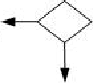
\includegraphics{./Images/Simbolos/simbolo-Decision.png}
\end{center}
\begin{enumerate}
  \item Almac\'en de Materia Prima: Si se tiene el stock disponible se registra la reserva de los materiales y se emite LE; caso contrario se emite LE con una fecha tentativa de ingreso de materia prima desde el proveedor, en forma simult\'anea se realiza una solicitud de compra seg\'un el Procedimiento del circuito de Compras (CNR).
  \item Almac\'en de Materia Prima: Si el PM es correcto entonces se procede a enviar el material; caso contrario lo devuelve a F\'abrica para que emita el PM nuevamente.
  \item F\'abrica: Si los materiales recibidos son los correctos se contin\'ua con la descarga; caso contrario se devuelven los materiales al Almac\'en de Materia Prima.
  \item F\'abrica: Si se recibe el AI se procede al env\'io de los materiales al Almac\'en de Producto Terminado. Si se recibe el NR, se comienza una serie de gestiones internas en funci\'on de Procedimientos est\'andares y manuales de autorizaciones, para el tratamiento de Producto NO CONFORME.
  \item Control de Calidad: Si la muestra pasa los controles de calidad, entonces se procede a emitir el IA; caso contrario se emite una NR.
\end{enumerate}

\begin{center}
  \textbf{Operación}
  
\includegraphics{./Images/Simbolos/simbolo-Operacion.png}
\end{center}
\begin{enumerate}
  \item Almac\'en de Materia Prima: Agrega en la columna correspondiente del formulario PM, la cantidad de materia prima que efectivamente se est\'e despachando.
\end{enumerate}

\begin{center}
  \textbf{Registro}
  
\includegraphics{./Images/Simbolos/simbolo-Registro.png}
\end{center}
\begin{enumerate}
  \item Planificaci\'on y Control de la Producci\'on: registra
  \item Almac\'en de Materia Prima: registra la reserva de materias primas en el LE.
  \item Almac\'en de Materia Prima: registra la salida de materia prima en la FSMP.
  \item Almac\'en de Producto Terminado: registra las cantidades recibidas de productos elaborados en la FSPT.
\end{enumerate}

\begin{center}
  \textbf{Almacenamiento definitivo}
  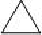
\includegraphics{./Images/Simbolos/simbolo-Almacenamiento-Definitivo.png}
\end{center}
\begin{enumerate}
  \item Planificaci\'on y Control de la Producci\'on: almacena de manera definitiva LRMP copia, OP tercera copia, LE original, PP original y NR original o IA original seg\'un corresponda.
  \item Almac\'en de Materia Prima: almacena de manera definitiva LE copia, LRMP original, PM original y primera copia conformada. 
  \item F\'abrica: almacena de manera definitiva PM tercera copia, PP tercera copia, OP original, PM segunda copia conformada y NR copia o IA copia seg\'un corresponda.
  \item Control de Calidad: almacena de manera definitiva OP primera copia, PP primera copia y IA segunda copia o NR segunda copia seg\'un corresponda.
  \item Almac\'en de Producto Terminado: almacena de manera definitiva OP segunda copia, IA primera copia y PP segunda copia.
\end{enumerate}

\begin{center}
  \textbf{Circuito no relevado}
  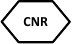
\includegraphics{./Images/Simbolos/simbolo-CNR.png}
  % simbolo-CNR.png: 73x44 pixel, 96dpi, 1.93x1.16 cm, bb=0 0 55 33
\end{center}
\begin{enumerate}
  \item Planificaci\'on y Control de la Producci\'on: Planificaci\'on.
  \item Almac\'en de Materia Prima: Compras.
  \item F\'abrica: Proceso Producci\'on.\
  \item F\'abrica: Tratamiento de Producto NO CONFORME.
\end{enumerate}

\pagebreak
\section{Formularios de Producci\'on}

\subsection{Orden de Producci\'on}
\begin{center}
 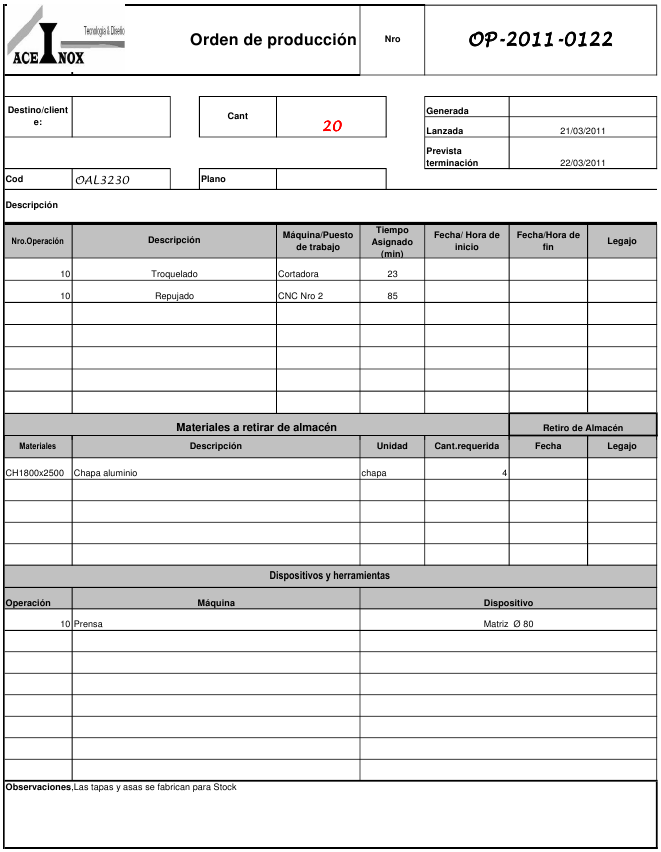
\includegraphics[scale=0.9,keepaspectratio=true]{./Circuitos-Teoricos/Produccion/Images/orden-de-produccion.png}
 % orden-de-produccion.png: 661x852 pixel, 96dpi, 17.49x22.54 cm, bb=0 0 496 639
\end{center}

\pagebreak
\begin{itemize}
 \item \textbf{Objetivo}: Es un documento en el que se especifican las operaciones que deben realizar la producci\'on.
 \item \textbf{Alcance}: Es un documento interno de la empresa.
\end{itemize}

\subsubsection{Descripción}
\begin{enumerate}
 \item Logo de la empresa.
 \item Número de Orden de Producci\'on.
 \item Cliente / Destino.
 \item Cantidad a realizar.
 \item Fecha de generaci\'on de la Orden de Producci\'on.
 \item Fecha de inicio de la producción.
 \item Fecha de finalización de la producción prevista.
 \item N\'umero de código interno de la producci\'on.
 \item N\'umero de plano.
 \item N\'umero de operaci\'on.
 \item Descripci\'on de la operaci\'on.
 \item M\'aquina o puesto de trabajo.
 \item Tiempo asignado (minutos).
 \item Fecha / Hora de inicio.
 \item Fecha / Hora de fin.
 \item N\'umero de legajo.
 \item C\'odigo del material a retirar por almac\'en.
 \item Descripci\'on del material a retirar por almac\'en.
 \item Unidad del material a retirar por almac\'en.
 \item Cantidad requerida del material a retirar por almac\'en.
 \item Fecha de retiro del material del almac\'en.
 \item Legajo de retiro del material del almac\'en.
 \item N\'umero de la operaci\'on donde se utilizar\'a dispositivos y herramientas.
 \item M\'aquina a utilizar.
 \item Dispositivo a utilizar.
 \item Observaciones.
\end{enumerate}

\pagebreak
\subsection{Hoja de Ruta}
\begin{center}
 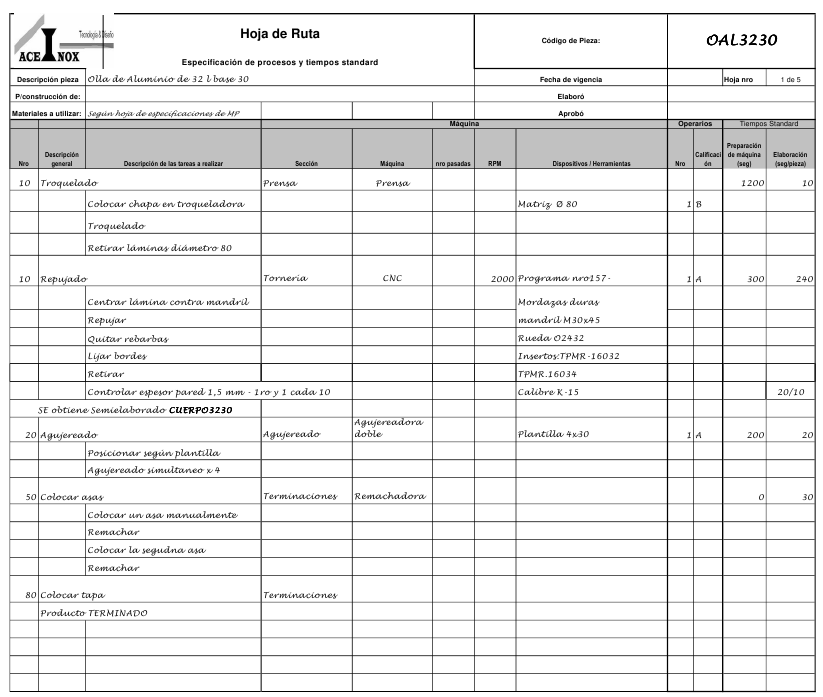
\includegraphics[angle=90,scale=0.95,keepaspectratio=true]{./Circuitos-Teoricos/Produccion/Images/hoja-de-ruta.png}
 % hoja-de-ruta.png: 823x697 pixel, 96dpi, 21.77x18.44 cm, bb=0 0 617 523
\end{center}

\pagebreak
\begin{itemize}
 \item \textbf{Objetivo}: Es un documento en el que se especifican las operaciones que se realizan sobre un mismo artículo hasta el momento de transformarlo en otro.
 \item \textbf{Alcance}: Es un documento interno de la empresa.
\end{itemize}

\subsubsection{Descripción}
\begin{enumerate}
 \item Logo de la empresa.
 \item C\'odigo interno de la pieza.
 \item Fecha de vigencia.
 \item Fecha de elaboraci\'on.
 \item Fecha de aprobaci\'on.
 \item Número de la hoja de ruta.
 \item Descripci\'on de la pieza.
 \item Pedido de construcci\'on.
 \item Materiales a utilizar.
 \item N\'umero de operaci\'on.
 \item Descripci\'on general.
 \item Descripci\'on de las tareas a realizar.
 \item Secci\'on de la m\'aquina. 
 \item Nombre de la m'aquina.
 \item N\'umero de pasadas por la m\'aquina.
 \item N\'umero de revoluciones por minuto para la m\'aquina.
 \item Dispositivos y herramientas.
 \item N\'umero de operario.
 \item Calificaci\'on del operario.
 \item Tiempo standard de preparacion de m\'aquina (segundos).
 \item Tiempo standard de elaboraci\'on (seg/pieza).
\end{enumerate}


\pagebreak
\section{Normas de control interno generales y específicas de Producci\'on}
\begin{itemize}
  \item \textbf{Existencia de inventario permanente o registros contables apropiados:} realización de recuentos físicos periódicos de las existencias, con toma de inventario rotativos, sorpresivos y realizados por personas ajenas a quienes detentan la custodia física de dichos bienes, y de quienes registran los movimientos de los mismos. El inventario físico contribuye a controlar y ajustar los movimientos físicos, evaluar la eficiencia operativa en el manejo de las existencias y sus registraciones, constatar la existencia física y controlar la imputación y valuación contable. Normalmente se debe efectuar un inventario físico total a fin del ejercicio contable.
  \item \textbf{Ajustes de inventario:} Los ajustes por diferencias de inventario deberán estar analizados, justificados y autorizados por un funcionario responsable que sea ajeno a la custodia de los bienes.
  \item \textbf{Custodia de las existencias:} La responsabilidad por la custodia y control de los bienes en existencia, debe recaer sobre una sola persona, a quien se le deben asegurar todas las facilidades de control. El local del depósito debe permitir una protección física adecuada de los bienes.
  Las condiciones del local deben garantizar que no se produzcan deterioros en los productos ( humedad, temperatura, ventilación, etc.)
  \item \textbf{Documentación de todo movimiento de existencias:} Todo movimiento de los bienes en Almacenes, debe estar amparado por el respectivo comprobante, debidamente firmado por un responsable con las atribuciones para realizar los respectivos movimientos.
  \item \textbf{Fijación de puntos de pedido, stocks mínimos y lotes óptimos:} Se recomienda la fijación de stocks de pedido, mínimos, máximos y lotes óptimos de pedido o criterios especiales de reaprovisionamiento.
  \item \textbf{Contratación de seguros adecuados}
\end{itemize}



\part{Cursogramas relevados de la empresa con la simbología correspondiente. Manual de cada cursograma relevado.}

\chapter{Circuito Compras}
%!!! cambiar esto por el diagrama de visio cuando este :)
\pagebreak
\section{Cursograma de Compras}
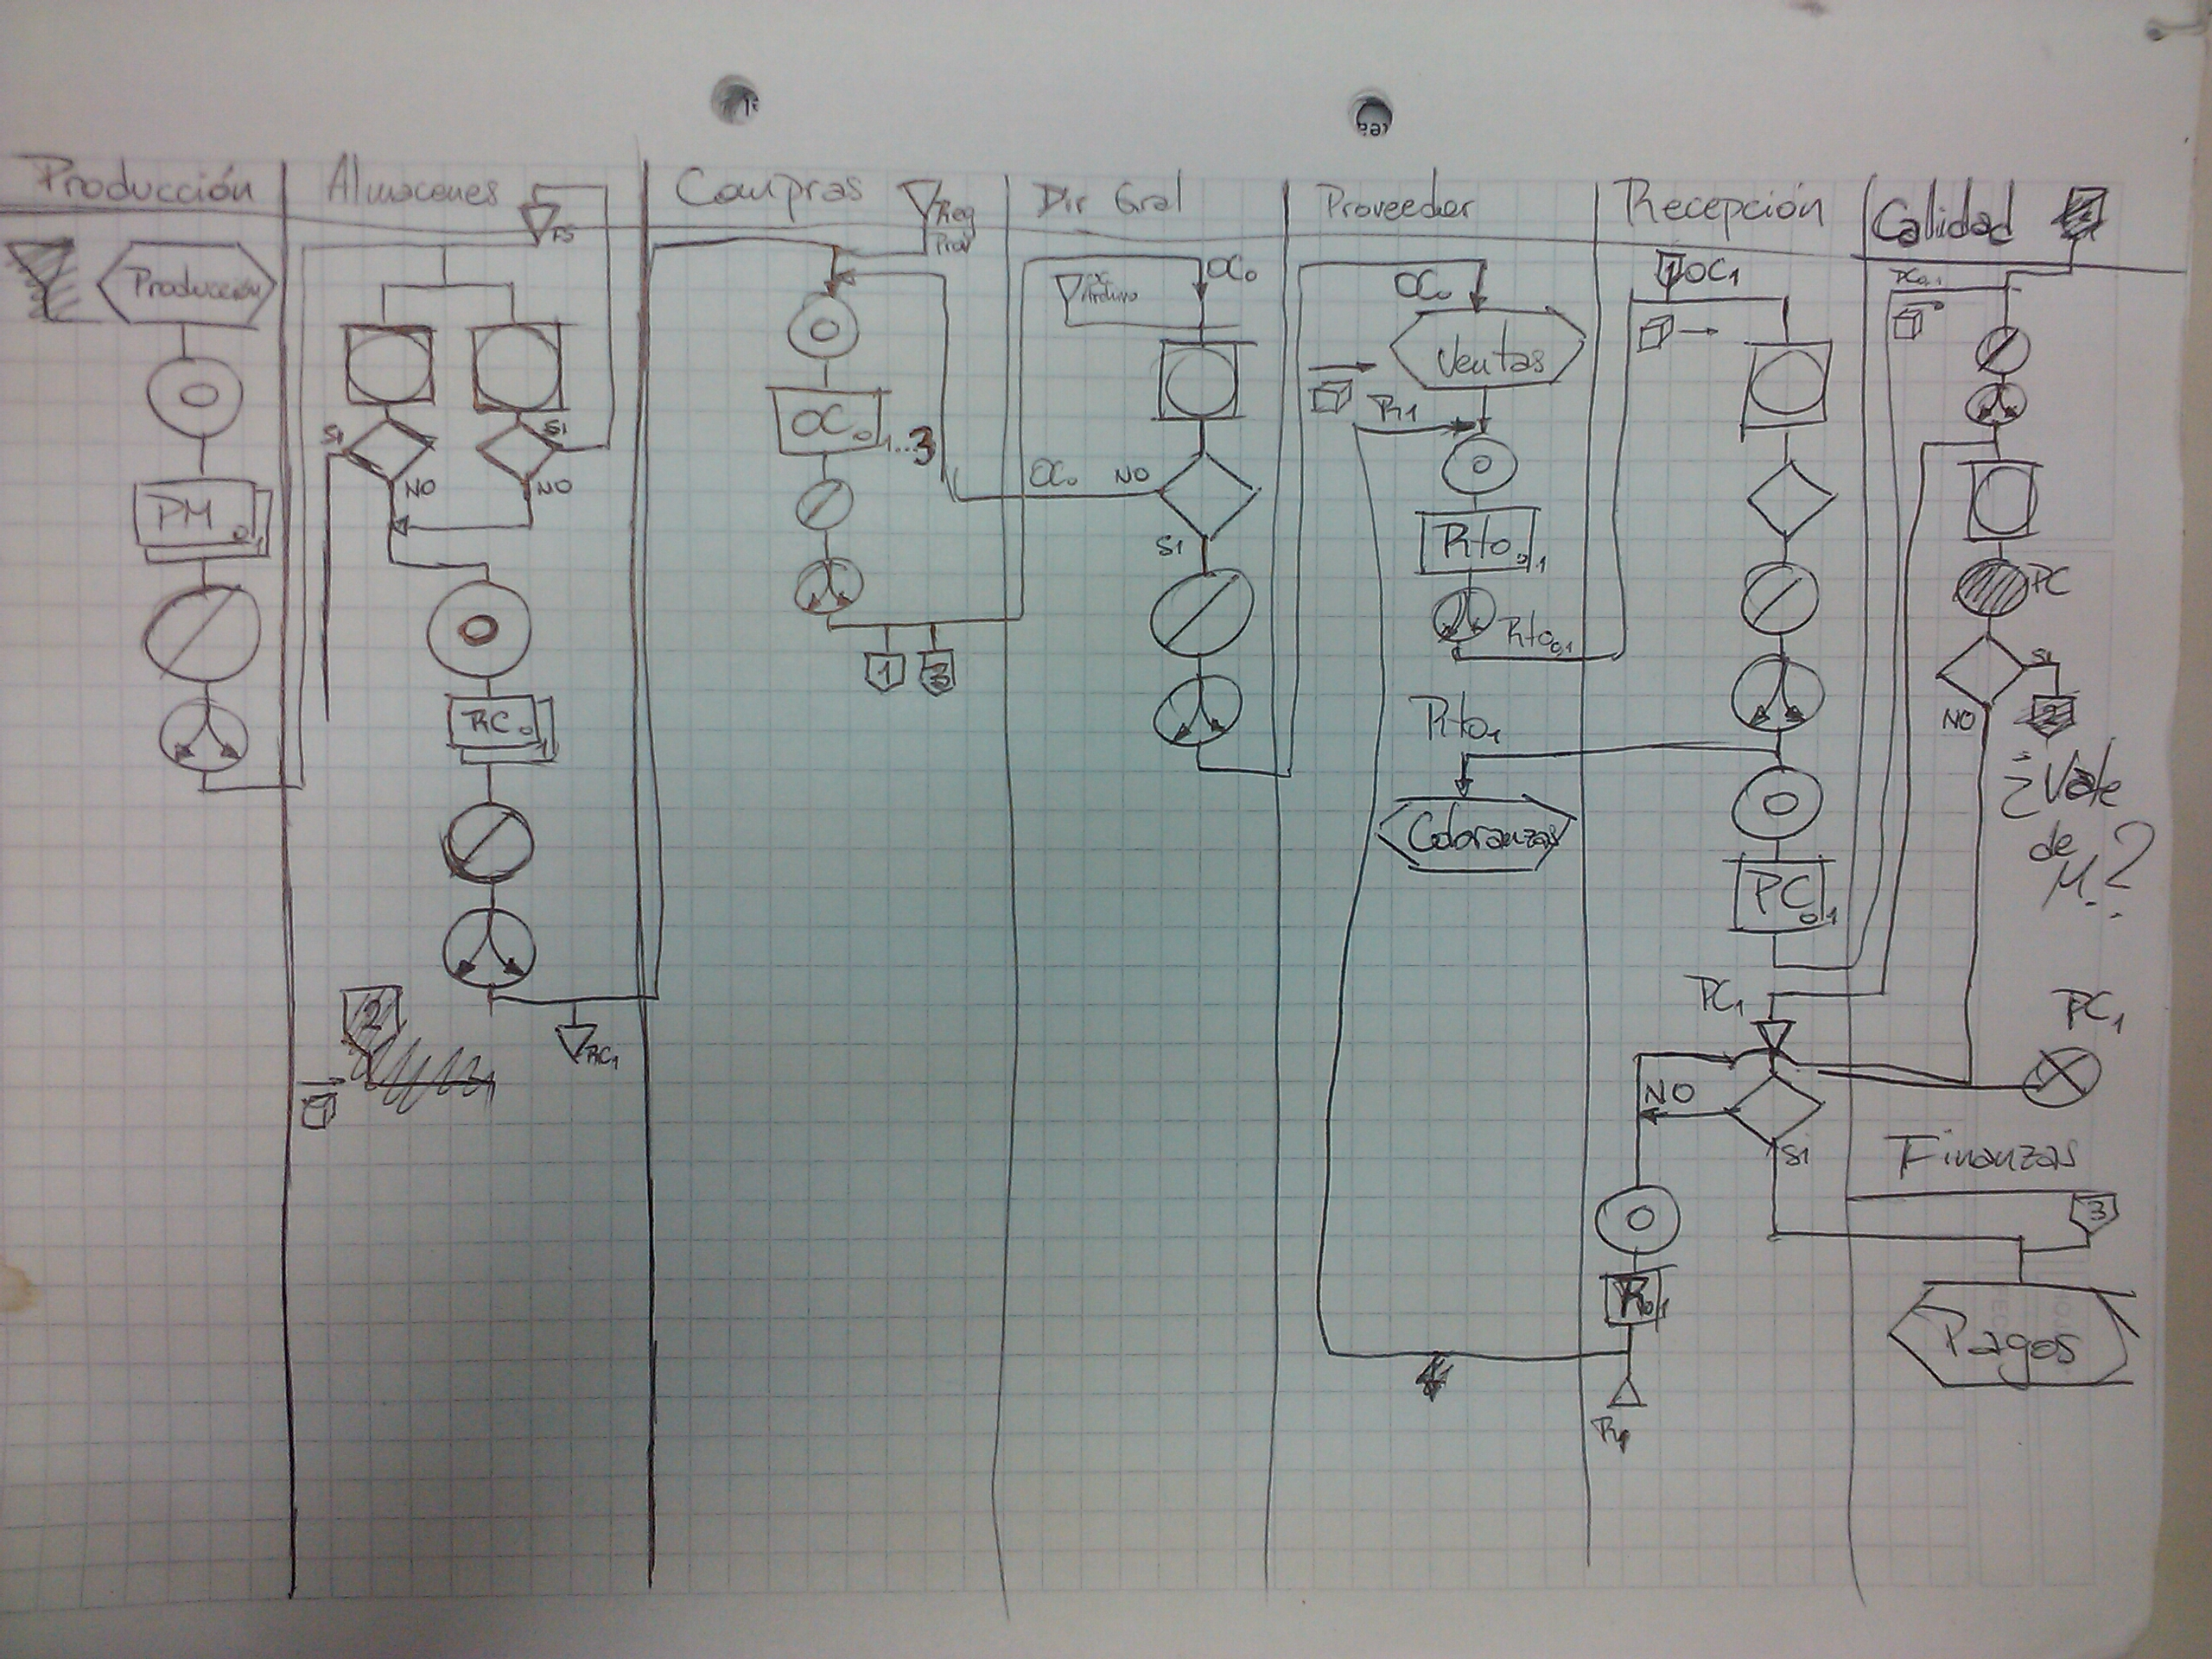
\includegraphics [scale=0.22 ,angle=90]{Empresa/Circuitos/Compras/Compras-v2.jpg}

\pagebreak
\section{Procedimiento de Compras}
\begin{description}
\item[Producción] Tras detectar necesidad de materiales el sector de Producción emite un Pedido de Materiales (PM) en original y copia, el nivel autorizante firma el original y lo envía al sector de Almacenes, se archiva la copia.
\item[Almacenes] Tras recibir Pedido de Materiales del sector de Producción, Almacenes chequea las existencias y si tiene materiales suficientes los despacha; si no tiene los materiales necesarios, o se alcanza el punto de pedido, Almacenes emite un Requerimiento de Compra (RC) en original y copia, lo firma y envía al sector de Compras el original archivando la compra.
\item[Compras] Recibido el Requerimiento de Compra, el área de Compras consulta listas de precios del Registro de Proveedores, confeccionadas con Pedidos de Cotización realizados mensualmente, y en función de ellos confecciona una Orden de Compra (OC) original y tres copias, las firma y distribuye original a Dirección General, una copia a Recepción, una a Finanzas, una a Calidad y almacena la última copia.
\item [Dirección General] Tras recibir la Orden de Compra del sector de Compras, la Dirección General controla los precios contra Ordenes de Compra archivadas de compras anteriores, y en caso de aprobarla la firma y envía al sector de Ventas del Proveedor previamente seleccionado. En caso de rechazarla devuelve la Orden de Compra al sector de Compras para su revisión.
\item [Proveedor] Una vez recibida la Orden de Compra firmada por Compras y Dirección General el, Proveedor, según su circuito de ventas,  decide aceptar o rechazar la Orden de Compra. En caso de aceptarla, el Proveedor confecciona Remito (Rto) por duplicado y envía original y una copia junto con los materiales al sector de Recepción.
\item[Recepción] Tras recibir los materiales y el Remito original y una copia, el sector de Recepción controla cotejando cantidades en ambos contra la Orden de Compra. En caso de concordar, firma Remito original y copia, almacena temporalmente el original y devuelve la copia al Proveedor. Emite Pedido de Control (PC) en original y copia, envía la mercadería al sector de Calidad para su control junto con ambas copias del documento.
\item [Proveedor] Recibido el remito firmado continua con su Circuito no relevado de Cobranzas.
\item [Calidad] Recibida la mercadería de Recepción firma la copia del Pedido de Control y lo devuelve a Recepción. Controla la calidad contra lo especificado en el Pedido de Control y registra en el mismo el resultado del control. De aprobar, envía la mercadería a Almacenes. De no aprobar, devuelve la mercadería a Recepción para su devolución al Proveedor. En ambos casos firma el Pedido de Control y la envía a Recepción.
\item [Recepción] Tras recibir el Pedido de Control original, si está rechazado emite un Reclamo en original y copia, envía el original al Proveedor junto con la mercadería y archiva el Pedido de Control y el Remito originales. Si está aprobada, envía el Remito original a Finanzas. En ambos devuelve la copia del Pedido de Control a Calidad, quien la destruye.
\item [Finanzas] Una vez recibido el Remito original del sector de Recepción, procede a realizar el pago en el circuito no relevado de Pago a Proveedores.
\end{description}


\pagebreak
\section{Cursograma de Compras (con numeración para el manual)}
IMAGENNNNNNNNNNNNNNNNNN

\pagebreak
\section{Manual del Cursograma de Compras}
\begin{center}\textbf{Sectores intervinientes}\end{center}
\begin{itemize}
  \item Producci\'on
  \item Almacenes
  \item Compras
  \item Direcci\'on General
  \item Proveedor
  \item Recepci\'on
  \item Control de Calidad
\end{itemize}

\begin{center}
  \textbf{Documentos}
  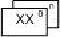
\includegraphics{./Images/Simbolos/simbolo-Documentos.png}
\end{center}
\begin{enumerate}
  \item Pedido de Materiales (PM)
  \item Orden de Compra (OC)
  \item Requerimiento de Compra (RC)
  \item Remito (RTO)
  \item Pedido de Control (PC)
  \item Reclamo (R)
\end{enumerate}

\begin{center}
  \textbf{Emisión de Documentos}
  
\includegraphics{./Images/Simbolos/simbolo-Emision-de-Documentos.png}
\end{center}

\begin{center}
  \textbf{Firma}
  
\includegraphics{./Images/Simbolos/simbolo-Firma.png}
\end{center}

\begin{center}
  \textbf{Distribución}
  
\includegraphics{./Images/Simbolos/simbolo-Distribucion.png}
\end{center}

\begin{center}
  \textbf{Almacenamiento Transitorio}
  
\includegraphics{./Images/Simbolos/simbolo-Almacenamiento-Transitorio.png}
\end{center}

\begin{center}
  \textbf{Control y verificación}
  
\includegraphics{./Images/Simbolos/simbolo-Control-y-Verificacion.png}
\end{center}

\begin{center}
  \textbf{Decisión}
  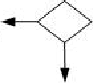
\includegraphics{./Images/Simbolos/simbolo-Decision.png}
\end{center}


\begin{center}
  \textbf{Registro}
  
\includegraphics{./Images/Simbolos/simbolo-Registro.png}
\end{center}

\begin{center}
  \textbf{Conector}
  
\includegraphics{./Images/Simbolos/simbolo-Conector.png}
\end{center}

\begin{center}
  \textbf{Almacenamiento definitivo}
  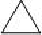
\includegraphics{./Images/Simbolos/simbolo-Almacenamiento-Definitivo.png}
\end{center}

\begin{center}
  \textbf{Circuito no relevado}
  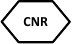
\includegraphics{./Images/Simbolos/simbolo-CNR.png}
  % simbolo-CNR.png: 73x44 pixel, 96dpi, 1.93x1.16 cm, bb=0 0 55 33
\end{center}

\pagebreak
\section{Formularios de Compras}
\subsection{Orden de Compra}
\begin{center}
 \includegraphics[scale=3.2, keepaspectratio=true]{./Images/FormulariosIEP/Orden-de-Compra.png}
 % Orden-de-Compra.png: 750x1002 pixel, 96dpi
\end{center}
\begin{itemize}
  \item \textbf{Objetivo:} Mediante este documento se comunica al proveedor la decisión de realizar una compra de materiales. Se especifican los productos a comprar con detalle de precios, cantidades, impuestos y condiciones de pago acordes a la previa cotización del proveedor.
  \item \textbf{Alcance:} Es un documento externo, entre la empresa y su proveedor.
  \item \textbf{Emisor:} Compras.
  \item \textbf{Cantidad de Copias Emitidas:} Original y cuatro copias.
  \item \textbf{Sector receptor:} Original a Dirección General para su autorización; primera copia a Recepci\'on; segunda copia a Finanzas; tercera copia a Control de Calidad; y la \'ultima copia a Compras.
 \end{itemize}
\subsubsection{Descripci\'on campos de la Orden de Compra}
\begin{enumerate}
  \item Empresa emisora: Raz\'on Social de la empresa.
  \item Empresa emisora: Informaci\'on de Sucursal. Domicilio y N\'umero de Tel\'efono.
  \item Empresa emisora: Responsabilidad frente al IVA.
  \item Número de Orden de Compra.
  \item Fecha de emisi\'on.
  \item Empresa emisora: CUIT y C\'odigo de Ingresos Brutos.
  \item Proveedor: Raz\'on Social.
  \item Proveedor: Domicilio.
  \item Proveedor: Responsabilidad frente al IVA.
  \item Condici\'on de pago.
  \item C\'odigo del proveedor al que se le compra.
  \item Proveedor: CUIT.
  \item Detalle de la Orden de Compra: C\'odigo del proveedor del \'item.
  \item Detalle de la Orden de Compra: Cantidad solicitada.
  \item Detalle de la Orden de Compra: Descripci\'on del \'item.
  \item Detalle de la Orden de Compra: Precio unitario del \'item.
  \item Detalle de la Orden de Compra: Importe total del \'item (cantidad * precio unitario).
  \item Detalle de la Orden de Compra: Fecha de entrega del \'item.
  \item Detalle de la Orden de Compra: Subtotal de items (suma de los totales de \'item).
  \item Resumen de la Orden de Compra: Subtotal de items (suma de los totales de \'item).
  \item Resumen de la Orden de Compra: Importe de impuestos que aplican (opcional).
  \item Resumen de la Orden de Compra: Subtotal después de impuestos (sólo si aplica impuestos).
  \item Resumen de la Orden de Compra: Gravamen de IVA para Inscriptos.
  \item Resumen de la Orden de Compra: Gravamen de IVA para No Inscriptos.
  \item Resumen de la Orden de Compra: Total después de IVA.
  \item Importe Total de la Orden de Compra.
  \item Importe Total de la Orden de Compra en letras.
  \item Fecha de Vencimiento de la Orden de Compra.
  \item Términos de confirmación de aprobación o rechazo.
\end{enumerate}

\pagebreak
\subsection{Requerimiento de Compra}
\begin{center}
 \includegraphics{Images/FormulariosIEP/Requerimiento-de-Compra.png}
 % Requerimiento-de-Compra.png: 493x299 pixel, 96dpi, 13.04x7.91 cm, bb=0 0 370 224
\end{center}

\begin{itemize}
  \item \textbf{Objetivo:} Un Requerimiento de Compra es un pedido interno entre sectores, para que el responsable de compras provea de algún elemento que un sector necesita.
  \item \textbf{Alcance:} Documento interno de la empresa.
  \item \textbf{Emisor:} Almacenes.
  \item \textbf{Cantidad de Copias Emitidas:} Original y copia.
  \item \textbf{Sector receptor:} Original a Compras; y la copia para Almacenes.
 \end{itemize}
\subsubsection{Descripci\'on campos del Requerimiento de Compra}
\begin{enumerate}
 \item Logo de la empresa.
 \item Nombre del formulario.
 \item N\'umero del Requerimiento de Compra.
 \item Departamento que solicita la Compra.
 \item Fecha en la que se realiza el Requerimiento de Compra.
 \item Fecha en la que se necesita los art\'iculos solicitados.
 \item Cantidad solicitada de un art\'iculo.
 \item Unidad de medida de un art\'iculo.
 \item Descripci\'on de un art\'iculo deseado.
 \item N\'umero del proveedor preferido (opcional).
 \item Firma del emisor.
\end{enumerate}


\pagebreak
\section{Normas de Control Interno de Compras}

\chapter{Circuito Ventas}
\pagebreak
\section{Cursograma de Ventas}
\begin{center}
 \includegraphics[scale=0.78,keepaspectratio=true]{Empresa/Circuitos/Ventas/Ventas-narrativa.jpg}
 % Ventas-narrativa.jpg: 847x1209 pixel, 96dpi, 22.41x31.99 cm, bb=0 0 635 907
\end{center}

\pagebreak
\section{Procedimiento de Ventas}
 \begin{description}
	\item[1 - Cliente] El cliente solicita un pedido emitiendo una 'Orden de Compra' (OC) mediante un 'Circuito No Relevado de Compras' (CNR Compras).
	\item[2 - Ventas] El \'area de ventas recibe la OC de parte del cliente y de esta manera genera la 'Solicitud de Pedido de Ventas' (SPV) especificando los detalles de la venta tal como est\'an especificados en la OC como por ejemplo, productos y plazo de entrega tentativo. Firma la SPV y env\'ia el original a Producci\'on y las copias a Almac\'en 1 y Contadur\'ia. Registra en el sistema la generaci\'on de la SPV y archiva en forma definitiva la 'Orden de Compra' junto a una copia de la SPV.
	\item[3 - Producci\'on] Producci\'on recibe la SPV y verifica que cuenta con stock suficiente. De no poseer stock necesario se procede a realizar el 'Circuito no relevado de de Producci\'on' (CNR Producci\'on). En caso de contar con el producto solicitado, genera una 'Orden de Pedido de Productos' (OPP) y la env\'ia a Almac\'en 2 (Almac\'en de roductos terminados).  Registra en el sistema la OPP y archiva en forma definitiva la SPV original y la copia de la OPP. 
	\item[4 - Almac\'en 2] Almac\'en 2 recibe la OPP, ya cuenta con el producto (ya sea porque ten\'ia stock o porque se ha producido especialmente) y env\'ia el producto junto con la documentaci\'on a Almac\'en 1. Registra en el sistema la actualización de la ficha de stock (FS) y el envío de productos al Almac\'en 1. Archiva definitivamente la OPP.
	\item[5 - Almac\'en 1] Almac\'en 1 prepara los productos para su entrega y genera el 'Remito' (RTO) correspondiente y tres copias. Entrega el producto al Transportista con el RTO original y entrega dos copias a Contadur\'ia. Registra en el sistema la generación de documentos y el env\'io de la mercader\'ia, y archiva en forma definitiva la 'Orden de Pedido de Productos' y una copia del Remito.
	\item[6 - Contadur\'ia] Contadur\'ia por un lado recibe la SPV asociada a la venta, y la archiva temporalmente. Al recibir el remito de Almac\'en 1 genera un listado de Remitos sin facturar asociados a la venta mediante el sistema, y emite la 'Factura'(F) correspondiente con dos copias. Registra en el sistema la emisi\'on de la factura y env\'ia el original y copia de la factura al Transportista para su env\'io al cliente. Contadur\'ia actualiza la Ficha de Cliente (FC) mediante el sistema y archiva definitivamente una copia de la factura y la SPV recibida.
	\item[7 - Transportista] Transportista recibe los remitos, las facturas y la carga a ser enviada. Env\'ia el pedido junto con la documentaci\'on al cliente. 
	\item[8 - Cliente] El cliente recibe los remitos, las facturas y el pedido. Chequea la mercader\'ia recibida junto con los documentos original, y firma las copias de los mismos. Distribuye las copias firmadas de vuelta a la empresa, y procede a realizar el 'Circuito No Relevado de Pagos' (CNR Pagos). Si la mercader\'ia no est\'a conforme a los pactado mediante la OC, se procede al CNR COmpras
	\item[9 - Almac\'en 1] Almacen 1 recibe la copia del remito firmado por el cliente, la registra en el sistema y lo archiva definitivamente. 
	\item[10 - Contadur\'ia] Contadur\'ia recibe la copia de la factura y el remito firmados por el cliente y la asienta la recepci\'on en el sistema. El pago de la factura es parte del 'Circuito no relevado de Cobranzas' (CNR Cobranzas)
\end{description}

\subsection{Entrevista}
Luego de analizar los diagramas de procedimiento de alto nivel del proceso de ventas que la empresa puso a nuestra disposici\'on, surgi\'o la necesidad de realizar una entrevista para aclarar ciertos puntos que no quedaban claros con nuestro contacto. Los puntos en cuesti\'on fueron los siguientes:
\begin{description}
 \item \underline{Ventas a Clientes}: \\
	Es el Centro de Atenci\'ion al Cliente (\textit{CAC}) quien interact\'ua con los clientes para realizar las ventas. Las ventas a clientes las ventas se realizan a partir de un pedido de cotizaci\'on confeccionado por el CAC. Posteriormente, el CAC formaliza el pedido de venta al recibir una Orden de Compra del cliente. Internamente, el CAC realiza una Solicitud de Pedido de Ventas (SPV).  \\
	Para el caso de los Distribuidores, ellos reciben la lista de precios y pueden formalizar directamente la Orden de Compra, es decir, que no hay cotizaci\'on previa del CAC.
 \item \underline{Registro de Clientes}: \\
	La empresa mantiene un registro de los clientes, y las transacciones que realizan con la empresa, mediante el sistema ERP Bejerman. Esta base de datos es actualizada por el \'area de Ventas, a trav\'es del \textit{CAC} y es consultada por todas las personas de la empresa que tienen habilitada esa funci\'on dentro de los m\'odulos del sistema inform\'atico. 
 \item \underline{Moviemiento de Materiales}: \\
	El medio de comunicaci\'on entre almacenes es electr\'onico, es decir, se realiza a trav\'es del sistema Bejerman, y as\'i se realizan las transferencias ``inter-dep\'osito''. Los documentos internos s\'olo se imprimen en papel cuando resulta necesario, y en casos particulares. En una \'epoca se utilizaban fichas y vale de materiales, pero fueron reemplazados por el sistema inform\'atico. Lo mismo sucede con el sector de Producci\'on, que maneja el movimiento de materiales mediante el sistema Bejerman.\\
	El sector de Producci\'on recibe por sistema la carga de datos del \'area de Ventas (CAC), formaliz\'andolo como ``Orden de Pedido''. En funci\'on a ello elabora una ``Orden de Montaje'', donde el sistema carga los elementos necesarios para confeccionar el pedido solicitado (las distintas partes y piezas para armar la luminaria). Terminado el producto, \'este se declara en el Dep\'osito Producto Terminado (02). Luego, el sector de Almacenes realiza por sistema la transferencia del producto, desde el 02 al Deposito Principal (01), y es desde aqu\'i que el \'area de Expedici\'on puede generar posteriormente el remito para despachar la mercader\'ia.  
	El transportista carga la mercader\'ia seg\'un la informaci\'on emanada de los remitos, controlando f\'isicamente la carga.  Luego se le confecciona una Hoja de Ruta con el itinerario diario y por ultimo se le emite un permiso ante el ARBA, en caso que la mercader\'ia que se transporte supere los \$20.000.-   
\end{description}

\pagebreak
\section{Cursograma de Ventas (con numeración para el manual)}
\begin{center}
 \includegraphics[scale=0.78,keepaspectratio=true]{Empresa/Circuitos/Ventas/Ventas-manual.jpg}
 % Ventas-manual.jpg: 847x1209 pixel, 96dpi, 22.41x31.99 cm, bb=0 0 635 907
\end{center}

\pagebreak
\subsection{Manual del Cursograma de Ventas}
\begin{center}\textbf{Sectores intervinientes}\end{center}
\begin{itemize}
  \item Cliente
  \item Ventas
  \item Producci\'on
  \item Almacen 2
  \item Almacen 1
  \item Contadur\'ia
  \item Transportista
\end{itemize}

\begin{center}
  \textbf{Documentos}
  \includegraphics{./Images/Simbolos/simbolo-Documentos.png}
\end{center}
\begin{enumerate}
  \item Orden de Compra (OC).
  \item Solicitud de Pedido de Ventas (SPV).
  \item Orden de Pedido de Productos (OPP).
  \item Remito (RTO).
  \item Factura (F).
\end{enumerate}

\begin{center}
  \textbf{Emisi\'on de Documentos}
  \includegraphics{./Images/Simbolos/simbolo-Emision-de-Documentos.png}
\end{center}
\begin{enumerate}
  \item Cliente emite una Orden de Compra (OC).
  \item Ventas emite una Solicitud de Pedido de Ventas (SPV) con 3 copias. 
  \item Producci\'on emite una Orden de Pedido de Productos (OPP) con duplicado.
  \item Almac\'en 1 emite Remitos (RTO) con 3 copias.
  \item Contadur\'ia emite Facturas (F) con 2 copias.
\end{enumerate}

\begin{center}
  \textbf{Firma}
  \includegraphics{./Images/Simbolos/simbolo-Firma.png}
\end{center}
\begin{enumerate}
  \item Ventas firma la Solicitud de Pedido de Ventas.
  \item Producci\'on firma la Orden de Pedido de Productos.
  \item Almac\'en 2 firma la Orden de Pedido de Productos.
  \item Cliente firma las copias de remito y factura.
\end{enumerate}

\begin{center}
  \textbf{Distribuci\'on}
  \includegraphics{./Images/Simbolos/simbolo-Distribucion.png}
\end{center}
\begin{enumerate}
  \item Ventas distribuye Solicitud de Pedido de Ventas a Producci\'on, Almac\'en 1 y Contadur\'ia.
  \item Producci\'on distribuye Orden de Pedido de Productos a Almac\'en 2.
  \item Almacen 2 distribuye los productos pedidos al Almac\'en 1.
  \item Almacen 1 distribuye los Remitos junto con el pedido al Transportista.
  \item Contadur\'ia distribuye las copias de los remitos y las facturas al Trasportista.
  \item Transportista distribuye los remitos, las facturas y el pedido al Cliente.
  \item El Cliente distribuye las copias de remito y facturas firmadas a Almac\'en 1 y a Contadur\'ia.
\end{enumerate}

\begin{center}
  \textbf{Almacenamiento Transitorio}
  \includegraphics{./Images/Simbolos/simbolo-Almacenamiento-Transitorio.png}
\end{center}
\begin{enumerate}
  \item Cliente almacena Orden de Compra.
  \item Almac\'en 1 almacena una copia de la SPV.
  \item Contadur\'ia almacena una ficha de cliente y la SPV.
  \item Transportista almacena los remitos, las facturas y el pedido.
\end{enumerate}

\begin{center}
  \textbf{Control y verificaci\'on}
  \includegraphics{./Images/Simbolos/simbolo-Control-y-Verificacion.png}
\end{center}
\begin{enumerate}
	\item Producci\'on controla si cuenta con stock suficiente con la Solicitud de Pedido de Ventas.
	\item El cliente controla si el pedido recibido es realmente lo que pidi\'o con la Orden de Compra.
\end{enumerate}
\pagebreak

\begin{center}
  \textbf{Decisi\'on}
  \includegraphics{./Images/Simbolos/simbolo-Decision.png}
\end{center}
\begin{enumerate}
  \item Producci\'on controla el stock. De no poseer procede a realizar el 'Circuito no relevado de de Producci\'on' (CNR Producci\'on). En caso de contar con el producto solicitado, genera una 'Orden de Pedido de Productos'.
  \item Cliente controla el pedido recibido. En caso de existir alg\'un inconveniente ejecuta parto de un 'Circuito no relevado de Compras', sino procede a la firma y distribuci\'on de los documentos firmados.
\end{enumerate}

\begin{center}
  \textbf{Registro}
  \includegraphics{./Images/Simbolos/simbolo-Registro.png}
\end{center}
\begin{enumerate}
  \item Ventas registra en el sistema la venta en curso y los documentos enviados.
  \item Producci\'on registra en el sistema la recepci\'on de la SPV y el env\'io de la OPP a Almac\'en 2.
  \item Almac\'en 2 registra en el sistema la recepci\'on de la OPP y la entrega de mercader\'ia a Almac\'en 1.
  \item Almac\'en 1 registra en el sistema la recepci\'on de la mercader\'ia la entrega de mercader\'ia.
  \item Contadur\'ia registra en el sistema la recepci\'on de SPV y los remitos, y la emisi\'on de la factura.
  \item Almac\'en 1 registra en el sistema el arribo de la copia del remito firmada por el cliente.
  \item Contadur\'ia registra en el sistema el arribo de la copia de la factura firmada por el cliente.  
\end{enumerate}

\begin{center}
  \textbf{Almacenamiento definitivo}
  \includegraphics{./Images/Simbolos/simbolo-Almacenamiento-Definitivo.png}
\end{center}
\begin{enumerate}
  \item Ventas almacena la Orden de Compra y una copia de la SPV.
  \item Producci\'on almacena la Solicitud de Pedido de Ventas y la copia de la OPP.
  \item Almac\'en 2 almacena la OPP.
  \item Almac\'en 1 almacena la copia de la SPV, una copia del remito y la copia firmada por el cliente del remito.
  \item Contadur\'ia almacena una copia de la factura y la copia de la factura y el remito firmada por el cliente.  
\end{enumerate}

\begin{center}
  \textbf{Circuito no relevado}
  \includegraphics{./Images/Simbolos/simbolo-CNR.png}
  % simbolo-CNR.png: 73x44 pixel, 96dpi, 1.93x1.16 cm, bb=0 0 55 33
\end{center}
\begin{enumerate}
  \item Compras (circuito del cliente).
  \item Pagos (circuito del cliente).
  \item Cobranzas.
\end{enumerate}

\pagebreak
\section{Formularios de Ventas}

\subsection{Factura}
\begin{center}
 \includegraphics[scale=0.85,keepaspectratio=true]{./Images/FormulariosIEP/Factura.png}
 % Factura.png: 749x973 pixel, 96dpi, 19.82x25.75 cm, bb=0 0 562 730
\end{center}
\begin{itemize}
  \item \textbf{Objetivo:} Con este documento se notifica al cliente que efectu\'o la compra el monto total a pagar. Se especifica el remito asociado, los productos comprados con detalle de precios, los impuestos incluidos y las condiciones de pago.
  \item \textbf{Alcance:} Es un documento entre la empresa y el cliente.
  \item \textbf{Emisor:} Contadur\'ia.
  \item \textbf{Cantidad de Copias Emitidas:} Original y Copia.
  \item \textbf{Sector receptor:} Expedici\'on, para su env\'io al cliente.
\end{itemize}
\subsubsection{Descripci\'on campos de la Factura}
\begin{enumerate}
  \item Empresa emisora: Raz\'on Social de la empresa
  \item Empresa emisora: Informaci\'on de Sucursal. Domicilio y N\'umero de Tel\'efono
  \item Empresa emisora: Responsabilidad frente al IVA
  \item Tipo de Factura (A en este caso)
  \item N\'umero de Factura
  \item Fecha de emisi\'on
  \item Empresa emisora: CUIT
  \item Empresa emisora: C\'odigo de Ingresos Brutos
  \item Empresa emisora: Fecha de inicio de actividades
  \item Cliente: Raz\'on Social 
  \item Cliente: Domicilio
  \item Cliente: Responsabilidad frente al IVA
  \item C\'odigo del cliente al que se le factura y C\'odigo de Vendedor (Opcional)
  \item Vencimiento de la Factura
  \item Condici\'on de entrega
  \item Cliente: CUIT
  \item Condici\'on de Venta / Tipo de Pago.
  \item Remito asociado a la Venta.
  \item Detalle de la factura: C\'odigo interno del \'item, Cantidad del \'item
  \item Detalle de la factura: Descripci\'on del \'item. La partida asociada es opcional
  \item Detalle de la factura: Precio unitario del \'item. El descuento del \'item es opcional.
  \item Detalle de la factura: Precio total del \'item (cantidad * precio unitario)
  \item Detalle de la factura: Subtotal de items (suma de los totales de \'item)
  \item Detalle de la factura: Detalle de Reg\'imenes Especiales que aplican.
  \item Total de Impuestos que aplican a la venta (sin IVA).
  \item Subtotal con Impuestos y sin IVA.
  \item IVA discriminado.
  \item Subtotal con Impuestos e IVA, sin Reg\'imenes Especiales.
  \item Total de Reg\'imenes Especiales.
  \item Total del Importe de la Factura.
  \item Importe de la factura en palabras.(Opcional)
  \item C\'odigo de Barras de la factura. El c\'odigo tambi\'en se encuentra en forma num\'erica. 
  \item Fecha de vencimiento del C\'odigo de Impresi\'on
  \item CAE: C\'odigo de Autorizaci\'on Electr\'onico.
  \item Copia de la facura: Original, Copia, Triplicado, etc
\end{enumerate}

\subsection{Remito}
\begin{center}
 \includegraphics[scale=0.90,keepaspectratio=true]{./Images/FormulariosIEP/Remito.png}
 % Remito.png: 713x959 pixel, 96dpi, 18.87x25.38 cm, bb=0 0 535 720
\end{center}
\begin{itemize}
  \item \textbf{Objetivo:} En este documento se detallan los productos a ser enviados al cliente. No se incluyen detalles de precios y se especifica la contidad de bultos.
  \item \textbf{Alcance:} Es un documento entre la empresa y el cliente.
  \item \textbf{Emisor:} Almac\'en 1.
  \item \textbf{Cantidad de Copias Emitidas:} Original y Copia.
  \item \textbf{Sector receptor:} Expedici\'on, para su env\'io al cliente.
 \end{itemize}
\subsubsection{Descripci\'on campos del Remito}

\begin{enumerate}

   \item Empresa emisora: Logo y Raz\'on Social de la empresa
   \item Empresa emisora: Domicilio Sucursal
   \item Empresa emisora: Domicilio Legal
   \item Empresa emisora: Informaci\'on de Contacto. N\'umeros de tel\'efono, sitio web, email, fax.
   \item Empresa emisora: Responsabilidad ante el IVA
   \item Tipo de Documento: Remito (S\'imbolo).
   \item Tipo de Documento: Remito.
   \item N\'umero de Remito.
   \item Fecha de Emisi\'on del Remito
   \item Empresa emisora: CUIT
   \item Empresa emisora: C\'odigo de Ingresos Brutos.
   \item Empresa emisora: Fecha de Inicio de Actividades.
   \item Cliente: Raz\'on Social
   \item Cliente: Domicilio 
   \item Cliente: Responsabilidad ante el IVA
   \item Cliente: C\'odigo interno de Cliente
   \item Solicitud de Pedido de Venta (SPV) asociada al remito.
   \item Cliente: Localidad
   \item Cliente: CUIT
   \item Detalle del Remito: C\'odigo de Producto.
   \item Detalle del Remito: Cantidad de Producto
   \item Detalle del Remito: Descripci\'on del Producto
   \item Detalle del Remito: Nota de Condici\'on de Entrega (Opcional)
   \item Detalle del Remito: Precio Total de la Mercader\'ia
   \item Cantidad de Bultos, Precio por Bulto, Flete y Seguro (Opcionales)
   \item Transportista: Nombre o Raz\'on Social
   \item Transportista: Domicilio
   \item Transportista: CUIT y Tel\'efono
   \item Fima Del Cliente
   \item Imprenta autorizada: Tel\'efono, CUIT, N\'umero de Inscripci\'on, Rango de Remitos Impresos.
   \item Imprenta autorizada: CAI. (C\'odigo de Autorizaci\'on de Imprenta)
   \item Vencimiento del Remito.
  \end{enumerate}
  
\pagebreak
\section{Normas de Control Interno de Ventas}
\begin{itemize}
 \item	{\bf Separaci\'on de funciones: } El encargado de ventas no debe poseer acceso a las registraciones de stock ni a la modificaci\'on de cuentas del cliente.
Quien vende no puede otorgar cr\'editos ni encargarse de la facturaci\'on. Dentro del sector de Ventas existe una clara divisi\'on entre la parte encargada de la atenci\'on a los clientes 
y la parte encargada de la venta en s\'i misma.
  \item	{\bf Aprobaci\'on de la venta: } Las pol\'iticas de ventas, otorgamiento de cr\'editos y precios son dispuestas por la Direcci\'on General.
La aprobaci\'on de la venta es realizada por el responsable de cr\'editos dado que es el que conoce el estado financiero de los clientes.
  \item	{\bf Movimiento de bienes: } La circulaci\'on de mercader\'ias est\'a respaldada por comprobantes firmados por el responsable del sector que los recibe. En los sectores de Producci\'on, 
Almac\'en 1 y 2 y Expedici\'on se documenta el transpaso de mercader\'ia utilizando el correspondiente m\'odulo del sistema inform\'atico de Bejerman.
  \item	{\bf Documentaci\'on prenumerada: } Toda documantaci\'on emitida debe estar prenumerada y se archivan en orden num\'erico, incluso las anuladas. Dado que todos los documentos se generan 
utilizando el sistema inform\'atico, resulta complicado alterar la numeraci\'on dado que la misma es autogenerada utilizando una secuencia.
  \item	{\bf Control de Facturaci\'on: } Contadur\'ia realiza un control cruzado de la facturaci\'on y remitos. Contadur\'ia siempre conserva una copia de las facturas y remitos emitidos. 
A su vez, realiza un control antes de que dichos documentos sean enviados al cliente.
\end{itemize}

\chapter{Circuito Cobranzas}
\pagebreak
\section{Cursograma de Cobranzas}
La empresa posee distintas formas de cobros, las cuales varian con el cliente. Algunas clientes pagan a traves de una cuenta corriente con una transferencia, otros con cheque o efectivo. A determinados clientes se les envía un cobrador mientras que muchos otros no.
Por simplicidad, en este caso se describe el caso en el cual el cliente se acerca a la empresa al sector de finanzas a entregar los valores (cheques o efectivo).

\includegraphics[scale=0.7]{Empresa/Circuitos/Cobranzas/cursograma-manual-cobranzas.jpg}

\pagebreak
\section{Procedimiento de Cobranzas}
\begin{enumerate}
  \item \textbf{Finanzas:} ejecuta un reporte en el sistema, el cual trae todas las facturas que vencen a la fecha. De ellas selecciona aquellas que no han sido pagadas. Esta tarea se realiza todos los días.
  Por cada factura vencida que no este paga, emite un reclamo del pago por duplicado, con una fecha de vencimiento de pago. El primero lo firma y se lo envía al cliente. El otro lo archiva para que quede constancia del reclamo.
  \item \textbf{Cliente:} recibe el reclamo o carta de documento, y en caso de pagar, confecciona un cheque para realizar el mismo y lo envia al sector de finanzas.
  \item \textbf{Finanzas:} en caso de recibir el cheque, revisa que corresponda con la cantidad a pagar y que este correctamente confeccionado. Si este esta correcto, emite un recibo por duplicado, firma el original y se lo entrega al cliente. Finalmente, archiva el cheque, la factura por triplicado, el duplicado del reclamo y registra en el sistema el pago de la factura.
  Si el cliente no paga, emite un reclamo a ventas y se lo envia a dicho sector. Si ya es la tercera vez que el cliente no paga, archiva los documentos utilizados y asienta en el sistema la falta de pago en la cuenta "pérdidas".
  \item \textbf{Ventas:} recibe el reclamo y si es la primera vez que se recibe un reclamo emite un segundo reclamo al cliente por duplicado. Firma el original y lo envia al cliente con una fecha límite para el pago. Si no es la primera vez que recibe un reclamo de finanzas, avisa de al sector legal de la falta de pago del cliente de manera informal(mail, llamado telefónico).
  \item \textbf{Legal:} una vez notificado de la falta de pago del cliente, emite una carta de documento, intimando al cliente a pagar las facturas que debe. La carta de documento es enviada al domicilio legal del cliente de forma tal que quede notificado.
\end{enumerate}

\pagebreak
\section{Manual del Cursograma de Cobranzas}

\begin{center}\textbf{Sectores intervinientes}\end{center}
\begin{itemize}
  \item Finanzas
  \item Ventas
  \item Cliente
  \item Legal
\end{itemize}

\begin{center}
  \textbf{Documentos}
  \includegraphics{./Images/Simbolos/simbolo-Documentos.png}
\end{center}
\begin{enumerate}
\item Reclamo a Cliente
\item Reclamo a Ventas
\item Cheque
\item Recibo
\item Carta Documento
\end{enumerate}

\begin{center}
  \textbf{Emisión de Documentos}
  \includegraphics{./Images/Simbolos/simbolo-Emision-de-Documentos.png}
\end{center}
\begin{enumerate}
\item Finanzas: Emite primer Reclamo a Cliente por original y copia.
\item Finanzas: Emite Recibo por original y copia.
\item Finanzas: Emite Reclamo a Ventas.
\item Cliente: Emite Cheque.
\item Ventas: Emite segundo y tercer Reclamo a Cliente por original y copia.
\item Legal: Emite Carta Documento por original y copia.
\end{enumerate}

\begin{center}
  \textbf{Firma}
  \includegraphics{./Images/Simbolos/simbolo-Firma.png}
\end{center}
\begin{enumerate}
\item Finanzas: Firma el original del primer Reclamo a Cliente.
\item Finanzas: Firma recibo oringinal con la entrega del cheque.
\item Finanzas: Firma el Reclamo a Ventas y se lo envia a dicho sector.
\item Cliente: Firma el cheque que luego entrega contra recibo a Finanzas.
\item Ventas: Firma el original del segundo o tercer Reclamo a Cliente.
\item Legal: Firma original de Carta Documento con la que notifica al cliente de la falta de pago.
\end{enumerate}

\begin{center}
  \textbf{Distribución}
  \includegraphics{./Images/Simbolos/simbolo-Distribucion.png}
\end{center}
\begin{enumerate}
\item Finanzas: distribuye el original del primer Reclamo a Cliente al cliente y conserva el duplicado.
\item Finanzas: entrega el recibo original a cambio del cheque recibido y conserva el duplicado del recibo.
\item Finanzas: distribuye el Reclamo a Ventas al sector de Ventas.
\item Cliente: entrega el cheque contra recibo.
\item Ventas: distribuye el original del segundo o tercer Reclamo a Cliente al cliente y conserva el duplicado.
\item Legal: Firma el original de Carta Documento y conserva el duplicado.
\end{enumerate}

\begin{center}
  \textbf{Almacenamiento Transitorio}
  \includegraphics{./Images/Simbolos/simbolo-Almacenamiento-Transitorio.png}
\end{center}
\begin{enumerate}
\item Finanzas: almacena copia del primer Reclamo a Cliente.
\end{enumerate}

\begin{center}
  \textbf{Control y verificación}
  \includegraphics{./Images/Simbolos/simbolo-Control-y-Verificacion.png}
\end{center}
\begin{enumerate}
\item Finanzas: Ejecuta un reporte en el sistema donde saca las facturas ya vencidas que no estan pagas. Controla el resultado del mismo con las factura por triplicado que tiene archivadas.
\item Finanzas: Verifica que el cheque que le fue entregado por el Cliente este correctamente confeccionado y se corresponda con el monto que indica la factura por triplicado que posee.
\item Finanzas: Luego de un tiempo controla si el Cliente pago o no el reclamo correspondiente. Verifica si el ya es el tercer reclamo que se le hizo al cliente.
\item Cliente: Verifica que sea correcta la factura que se le esta reclamando, y que se corresponda con lo que el mismo posee en sus registros y documentos.
\item Ventas: Ventas verifica si es el primer o segundo reclamo que le ha llegado por parte de una misma factura de ese cliente.
\end{enumerate}

\begin{center}
  \textbf{Decisión}
  \includegraphics{./Images/Simbolos/simbolo-Decision.png}
\end{center}
\begin{enumerate}
\item Finanzas: Una vez que el resultado del reporte de facturas vencidas y que estas esten correctas emite los correspondientes reclamos para el cliente. Si no, no hace nada ( no hay facturas a cobrar).
\item Finanzas: Si el cheque recibido esta bien hecho y se corresponde con el monto de la factura vencida, procede a emitir el recibo correspondiente. Si el cliente no paga, venciendose el plazo de la factura o reclamo, procede a verificar si ya se han emitido otros reclamos o no.
\item Finanzas: Si ya era el tercer reclamo que se le envio al cliente, procede a asentar la falta de pago en el sistema. Si no, emite el primer o segundo reclamo correspondiente a Ventas.
\item Cliente: Una vez verificada la factura que se le reclama decide en caso de estar correcta la misma, confeccionar el cheque para realizar el pago. En caso contrario no hace nada (o depende de cada cliente, en realidad no interesa que hace si no paga).
\item Ventas: Una vez verificado el reclamo proveniente de Finanzas, y que este este correcto emite un Reclamo a Cliente. Si este no era el primer reclamo que venia del sector de Ventas, notifica de la falta de pago a Legal para que emita la Carta Documento.
\end{enumerate}

\begin{center}
  \textbf{Registro}
  \includegraphics{./Images/Simbolos/simbolo-Registro.png}
\end{center}
\begin{enumerate}
\item Finanzas: registra en el sistema el cobro en la cuenta "cobros".
\item Finanzas: registra en el sistema el la falta de pago en la cuenta "pérdidas".
\end{enumerate}

\begin{center}
  \textbf{Almacenamiento definitivo}
  \includegraphics{./Images/Simbolos/simbolo-Almacenamiento-Definitivo.png}
\end{center}
\begin{enumerate}
\item Finanzas: archiva el cheque, el duplicado del recibo, el duplicado del primer Reclamo a Cliente y el triplicado de la factura.
\item Finanzas: archiva el duplicado del primer Reclamo a Cliente, el duplicado del primer y segundo Reclamo a Ventas y el triplicado de la factura.
\item Cliente: archiva el original del recibo.
\item Ventas: almacena copia del segundo y/o tercer Reclamo a Cliente.
\item Legal: almacena copia de Carta Documento.
\end{enumerate}

\pagebreak
\section{Formularios de Cobranzas}
\subsection{Formulario1}
imagen
\begin{itemize}
  \item \textbf{Objetivo:}
  \item \textbf{Alcance:}
  \item \textbf{Emisor:}
  \item \textbf{Cantidad de Copias Emitidas:}
  \item \textbf{Sector receptor:}
 \end{itemize}
\subsubsection{Descripci\'on campos del Formulario1}

\subsection{Formulario2}
imagen
\begin{itemize}
  \item \textbf{Objetivo:}
  \item \textbf{Alcance:}
  \item \textbf{Emisor:}
  \item \textbf{Cantidad de Copias Emitidas:}
  \item \textbf{Sector receptor:}
 \end{itemize}
\subsubsection{Descripci\'on campos del Formulario2}

\pagebreak
\section{Normas de Control Interno de Cobranzas}


\part{Presupuesto}

% ANEXOS
\appendix
\chapter{Ap\'endice 1: Diagramas de información entregado por la empresa}
{\large{Compra de materiales}} \\
{\bf{Descripción:}} \\
Flujo operativo cuando se realiza una solicitud de compra de materiales. Este proceso va desde el origen de la necesidad de compra, hasta que se realiza el pago de la misma. \\

{\large{Control de entradas de inventario}} \\
{\bf{Descripción:}} \\
Definir exactamente los pasos que deben hacerse para ingresar un producto en elstock de la empresa. \\

{\large{Pedido de venta de producto, transporte propio}} \\
{\bf{Descripción:}} \\
Flujo operativo cuando un cliente realiza un pedido de ventas, y en su expedición se utiliza un transportista contratado por nosotros mismos. \\

{\large{Proceso de cobro de facturas}} \\
{\bf{Descripción:}} \\
Flujo operativo de un cobro de factura. En el proceso actual hay una serie de particularidades, como cheques posdatados (que pueden endosarse para pagar proveedores), y otros documentos de compra que pueden utilizarse para aplicar cobros de clientes.


\begin{center}
 \includegraphics[angle=90,scale=0.80,keepaspectratio=true]{./Images/Procesos-Circuitos-Originales-IEP/Circuito-Compras-IEP.png}
 % Circuito-Compras-IEP.PNG: 1024x768 pixel, 96dpi, 27.10x20.32 cm, bb=0 0 768 576
\end{center}

\begin{center}
 \includegraphics[angle=90,scale=0.80,keepaspectratio=true]{./Images/Procesos-Circuitos-Originales-IEP/Circuito-Compras2-IEP.png}
 % Circuito-Compras2-IEP.PNG: 1024x768 pixel, 96dpi, 27.10x20.32 cm, bb=0 0 768 576
\end{center}

\begin{center}
 \includegraphics[angle=90,scale=0.80,keepaspectratio=true]{./Images/Procesos-Circuitos-Originales-IEP/Circuito-Ventas-IEP.png}
 % Circuito-Ventas-IEP.PNG: 1024x768 pixel, 96dpi, 27.10x20.32 cm, bb=0 0 768 576
\end{center}

\begin{center}
 \includegraphics[angle=90,scale=0.80,keepaspectratio=true]{./Images/Procesos-Circuitos-Originales-IEP/Circuito-Cobranzas-IEP.png}
 % Circuito-Cobranzas-IEP.PNG: 1024x768 pixel, 96dpi, 27.10x20.32 cm, bb=0 0 768 576
\end{center}


% ------------------------------ Fin del tp -------------------------------

\end{document}

%---------------------------- Fin del documento ---------------------------
